\documentclass[10pt,journal,compsoc]{IEEEtran}

\ifCLASSOPTIONcompsoc
  % IEEE Computer Society needs nocompress option
  % requires cite.sty v4.0 or later (November 2003)
  \usepackage[nocompress]{cite}
\else
  % normal IEEE
  \usepackage{cite}
\fi

\usepackage{algorithm,setspace}
\usepackage[noend]{algpseudocode} % needed for: algorithm pseudocode
\usepackage{color}
\usepackage{array}
\usepackage{multirow}
\usepackage{amsmath}
\usepackage{amssymb}
\usepackage{graphicx}
\usepackage{url}
\usepackage{hyperref}
\usepackage{stmaryrd}
\usepackage{soul}
\usepackage{cancel}
\usepackage{listings}
\usepackage{tikz} % needed for: tikz pics
\usetikzlibrary{arrows}
\usetikzlibrary{decorations.pathreplacing}

\definecolor{aliceblue}{rgb}{0.94, 0.97, 1.0}
\definecolor{applegreen}{rgb}{0.55, 0.71, 0.0}
\definecolor{amber}{rgb}{1.0, 0.75, 0.0}

\lstdefinestyle{mystyle}{
	tabsize          = 1,     % tab space width
	numbers          = left,  % display line numbers on the left
	%stepnumber		 = 2,
	numberfirstline=false,
	%framesep         = 1pt,   % expand outward
	framerule        = 0.2pt, % expand outward 
	commentstyle     = \color{applegreen},      % comment color
	keywordstyle     = \color{blue},       % keyword color
	stringstyle      = \color{amber},    % string color
	backgroundcolor  = \color{aliceblue}, % backgroundcolor color
	showstringspaces = false,              % do not mark spaces in strings
	otherkeywords	 ={signal,inos_task,uint16_t},
	language = C,
	%numbers = none, 
	escapechar = !,
	basicstyle = \ttfamily\bfseries\scriptsize, 
	xleftmargin=0.5ex,
	linewidth = .75\linewidth,
	basicstyle=\tiny,
}

\newcommand{\expected}[1]{E\!\left\llbracket #1 \right\rrbracket}
\newcommand{\revised}[1]{\textcolor{blue}{#1}}
\newcommand{\TODO}[1]{\textcolor{blue}{\textbf{TODO: }}\textcolor{red}{#1}}
\newtheorem{fact}{Fact}

% text revision commands
\newcommand{\add}[1]{\textcolor{blue}{#1}}
\newcommand{\remove}[1]{\textcolor{red}{\st{#1}}}
\newcommand{\replace}[2]{\remove{#1} \add{#2}}


\begin{document}

\title{On the Synchronization of Computational RFIDs}

\author{Kas{\i}m~Sinan~Y{\i}ld{\i}r{\i}m, 
	Henko~Aantjes, 
	Przemys{\l}a~Pawe{\l}czak~\IEEEmembership{Member,~IEEE,} 
	and~Amjad~Yousef~Majid
	%
	\IEEEcompsocitemizethanks{
		\IEEEcompsocthanksitem A preliminary version of this article was presented at the HLPC 2016 Workshop, Atlanta, GA, USA, April 2, 2016~\cite{hlpc2016}. \protect\\
		\IEEEcompsocthanksitem The authors are with the Embedded Software Group, Delft University of Technology, Mekelweg 4, 2628 CD Delft, The Netherlands (e-mail: \{k.s.yildirim, p.pawelczak, a.y.majid\}@tudelft.nl, h.aantjes@student.tudelft.nl).
	}
%	\thanks{Manuscript received April 19, 2005; revised August 26, 2015.}
}


\IEEEtitleabstractindextext{%
\begin{abstract}
Battery-free computational RFID platforms, such as WISP (Wireless Identification and Sensing Platform), are intermittently-powered devices designed for replacing existing sensor networks. Accordingly, synchronization appears as one of the  crucial building blocks for collaborative and coordinated actions in these platforms. However, intermittent power leads to frequent loss of computational state and short-term clock frequency instability that makes synchronization challenging. In this article, we introduce WISP-Sync protocol that provides synchronization among WISP tags in the communication range of an RFID reader. WISP-Sync overcomes the aforementioned challenges by employing a Proportional-Integral (PI) controller-inspired algorithm which (i) is adaptive---reactive to short-term clock instabilities; (ii) requires only a few computation steps---suitable for limited harvested energy; and (iii) keeps a few variables to hold the synchronization state---minimum overhead to recover from power interrupts.	Evaluations in our testbed showed that WISP-Sync ensured an average synchronization error of approximately 1\,ms among the tags with an average energy overhead of 1.85\,$\mu$J per synchronization round.
\end{abstract}

% Note that keywords are not normally used for peerreview papers.
\begin{IEEEkeywords}
Time Synchronization, Computational RFIDs, Wireless Identification and Sensing Platform (WISP).
\end{IEEEkeywords}}

\maketitle

\IEEEdisplaynontitleabstractindextext

\IEEEpeerreviewmaketitle



\IEEEraisesectionheading{\section{Introduction}\label{sec:Intro}}

\IEEEPARstart{L}{ow-power} wireless embedded systems consist of tiny, low-cost and spatially separated computers that communicate with each other by exchanging radio packets. Powering these small-scale embedded systems, e.g. wireless sensor networks (WSNs), is still a crucial problem~\cite{emergence}. Replacing or recharging their batteries is impractical and inhibits long-term operation. Moreover, batteries increase the size and cost of the hardware. Fortunately, the energy efficiency of these systems has improved considerably such that their power requirements are in the order of a few $\mu$W \cite{booksmith2013}. Furthermore, recent advancements in microelectronics technology enabled harvesting power from radio frequency (RF) sources that is sufficient to operate low-power embedded systems in practice~\cite{60ghz,emergence,bi:commag:2015,xie_wcom_2013,garnica_procieee_2013}. Nowadays, the growth of the RF-powered computing paradigm is bringing new research opportunities and challenges~\cite{emergence}, leading to a promising class of low-power embedded systems, the so-called Intermittently Powered Devices (IPDs).

By taking existing RFID (Radio Frequency IDentification) technology as a foundation, computational RFIDs (CRFIDs) are emerging IPDs that allow sensing, computation and communication without batteries---replacing existing battery-powered sensor networks~\cite{booksmith2013}. CRFIDs are equipped with a backscatter radio~\cite[Chapter 4]{rfid_handbook} composed of a simple circuitry that modulates the carrier wave generated by a reader to transmit information. This allows communication to come almost for free. This is a fundamental difference from sensor networks where the transceiver circuit is the most energy-hungry component. In the CRFID domain, the bottleneck in terms of power consumption has shifted from communication to computation and sensing~\cite{ekhonet}. A typical example of CRFIDs is the WISP (Wireless Identification and Sensing Platform)~\cite{wisp}. Commercial RFID readers implementing the EPC Gen2 standard~\cite{epc_gen2} are used to power WISP tags. Apart from low data rate sensing~\cite{neuralWISP}, these maintenance-free devices are evolving to support high data rate and more complex sensing applications such as continuous sensor-data streaming, e.g. capture and transfer of images via battery-free cameras, i.e. WISPCam~\cite{wispcam_2015,cameralocalize_2015}.

\subsection{The Need for CRFID Network Synchronization}

As of now, battery-less networks are in the form of one-hop architecture in which the CRFID tags communicate only with the RFID reader~\cite{wisp,booksmith2013,wisent:2016}. \add{Therefore, CRFID tags cannot operate in a multi-hop manner.} However, recent advancements in the wireless communication enabled tag-to-tag communication, e.g.~\cite{liu2013ambient}.  We anticipate that \add{this communication capability will lead up multi-hop CRFID networks that} will demand their own implementation of basic sensor network building blocks~\cite{levis:tinyos} with the aim of replacing the existing battery-powered sensing and data collection applications with their battery-less counterparts. 

\add{Since we are not aware of any network infrastructure demonstrating neither multi-hop communication nor multi-hop synchronization, our focus in this article are the CRFID networks where several readers cover a tag population simultaneously in a single hop. A representative application is the greenhouse monitoring where several tags are powered by multiple readers, see Figure~\ref{fig:motivation}. In this application, the tags sense the environment and timestamp their temperature readings. When the readers request their temperature readings, the tags transmit their timestamps together with the collected temperature data. In order to make inferences on the collected temperature readings, timestamps should be consistent so that the readers can provide a temporal ordering of the readings. Therefore, tags require a common time notion to timestamp their readers---creating a demand for explicit time synchronization. In order to achieve synchronization, readers should first acquire the global time, e.g. by accessing time servers using the Internet; then individual tags should be synchronized to the individual readers.}

%We conjecture that in this new battery-less sensing architecture the synchronization will be a fundamental building block that allows, for instance, temporal ordering of the collected data in order to make inferences at the CRFID tag side. Therefore, establishing a common time notion among the tags, rather than synchronizing RFID readers only, will be a crucial service.

\begin{figure}
	\centering
	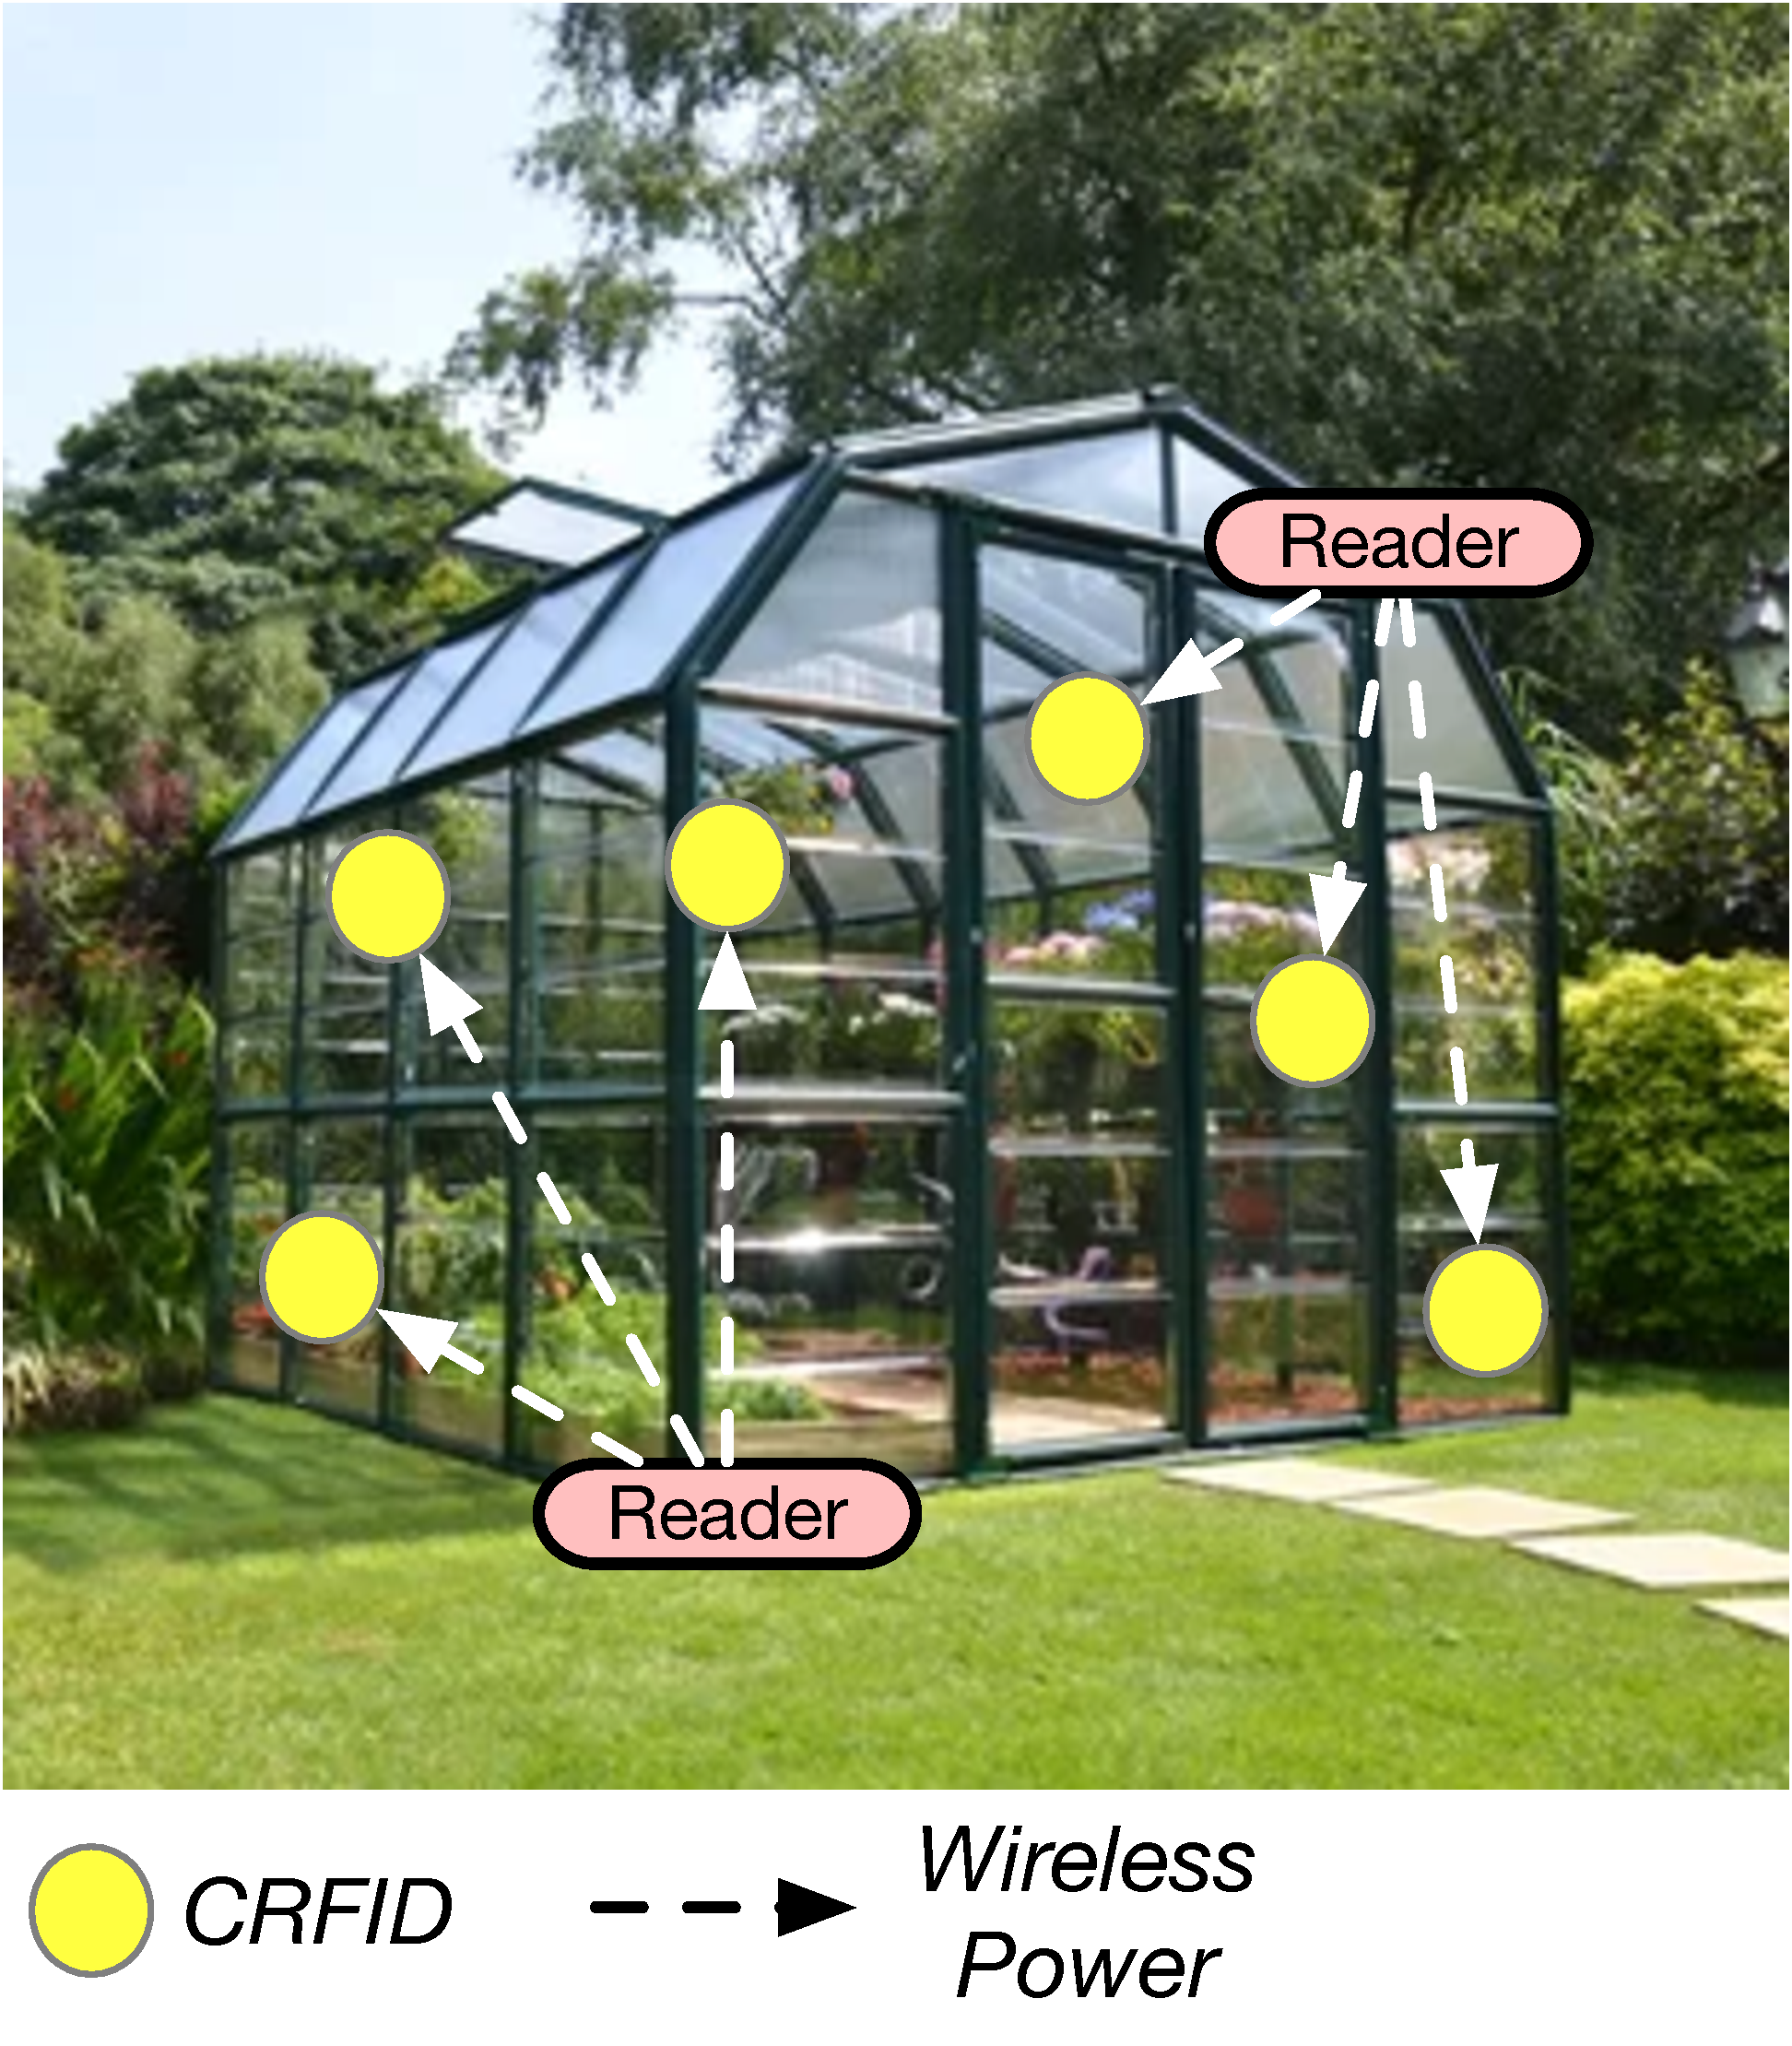
\includegraphics[width=0.75\columnwidth]{figures/scenario.pdf}
	\caption{\label{fig:motivation}\color{blue}A representative greenhouse monitoring application using CRFIDs. Two readers are deployed to provide power to the individual tags and to collect their periodic sensor readings.}
\end{figure}

\subsection{Differences From Battery-Powered WSNs }
\label{sec:Motivation}

\add{The EPC Gen2 protocol uses slotted Aloha that performs a form of synchronization between the reader and the tags: by adjusting clock offset differences and introducing guard times, tags are ensured to communicate at the allocated slot boundaries. However, this method does not compensate for clock drifts and output a synchronized clock value that can be accessed by the tags to timestamp (and make inference about) the collected information, e.g. from the sensors attached to tags. In consequence, applications requiring time notion cannot be enabled, since a clock should be maintained at each tag---making synchronization service mandatory. However, the characteristics of CRFID systems expose fundamentally different challenges than battery-powered sensor networks to implement the synchronization service. The reason is mainly twofold:}

\begin{itemize}
	\item \textbf{Challenge I:} CRFID systems should perform computations efficiently using \emph{marginal} and intermittent RF power that leads to frequent loss of computational state, e.g. when the RFID reader moves away from the CRFID tag \cite{ransford:2008}. Therefore, computations pertaining to time synchronization have an extremely short time budget, e.g. should be completed with the other computation tasks within 10--100\,ms in WISP~\cite{Ransford:2011:Mementos}. On the contrary, the synchronization approaches in WSNs, e.g. the de facto protocol \cite{Maroti2004}, keep communication infrequent by pushing computation instead, so that the battery power is used efficiently in order to extend the life-time of the network up to several years.
	
	\item \textbf{Challenge II:} The continuously varying voltage supply introduces severe hardware instability, e.g. varying oscillator frequencies in short-term affects the stability of the clocks and degrades the accuracy sensing. Therefore, computations pertaining to time synchronization should be reactive against very-frequent voltage effects; e.g. during super-capacitor discharge. On the contrary, in WSNs the input voltage is constant and the temperature is the main factor affecting the clock frequencies~\cite{schmid2010interaction}. Temperature compensation techniques, e.g. \cite{Schmid:2009}, are not applicable to compensate for the voltage instabilities in CRFIDs due to their computational complexity.	
	
\end{itemize}

\subsection{Contributions}

The focus of this article is to answer the question of \emph{how to design a building block that synchronizes intermittently-powered CRFID systems?} To this end, we investigate the WISP platform and provide initial observations and limitations pertaining to the synchronization of these devices. In particular, the main contributions and findings of 
this article are:
%
\begin{itemize}
	\item To the best of our knowledge, this is the first study that focuses on the synchronization of tags in CRFID systems. Even though there are studies on the synchronization of multiple RFID readers, e.g.~\cite{reader_sync}, we are unaware of any study that provides synchronization of individual tags in the communication range of an RFID reader. 
	\item By addressing the aforementioned challenges, we design and implement \emph{the first synchronization primitive} for the tags, namely \emph{WISP-Sync}, inspired by the Proportional-Integral (PI) controllers~\cite{pi2015,yildirim2017adaptive}. WISP-Sync (i) 
	requires only a few computation steps to run efficiently under limited harvested energy and keeps a few variables to hold the synchronization state to recover from power interruptions with minimum overhead---\emph{addressing Challenge I}; (ii) is adaptive to react to clock instabilities in a fast manner---\emph{addressing Challenge II}.
	\item \add{Our time synchronization algorithms compensate for the clock drift and enable the first step to enable an \emph{explicit clock} for CRFID applications. Moreover, our implementations are independent of how EPC Gen2 is implemented---providing a level of portability across different platforms.}
	%
	\item We provide theoretical analysis to prove that this primitive establishes synchronization and to reveal the factors affecting its synchronization performance.
	%
	\item Evaluations in our testbed show that an average synchronization error of approximately 1\,ms can be ensured among tags with an energy overhead of 1.85\,$\mu$J per synchronization round using this  primitive.
\end{itemize}
%
We note that WISP-side implementations throughout the article are done using C and assembly language. All source codes and scripts used to generate the results in the article (including parsing, post-processing and measurement results) are available via~\href{https://goo.gl/RuWIZ2}{https://goo.gl/RuWIZ2}.

The remainder of this article is organized as follows. In Section~\ref{sec:Related-Work} we present the fundamental challenges of synchronizing IPDs. Section~\ref{sec:Clock_Hardware} presents the hardware, in particular clock system of the WISP platform briefly, while Section~\ref{sec:clock_model} provides the mathematical notation to be used throughout the article. In 
Section~\ref{sec:sender_receiver} we propose a sender-receiver synchronization approach between an RFID reader and a single tag. Sections~\ref{sec:event_based} and~\ref{sec:eval-wispsync} present the WISP-Sync protocol and its evaluation in our testbed, respectively. We also present the synchronization of multiple tags in Section~\ref{sec:multi-wisp}. Finally, we provide our conclusions and future research directions in Section~\ref{sec:Conclusion}.  

\section{Synchronizing Battery-Free CRFIDs}
\label{sec:Related-Work}

In this section, we present a brief  state of the art on synchronization issues in conventional WSNs. Then, we emphasize the main challenges of synchronizing wireless battery-free embedded systems by focusing on a particular IPD platform: computational RFIDs. 

\subsection{Synchronization in Conventional WSNs}
\label{sec:WSN-Sync}

The instability of the clock hardware, delays during communication among sensor nodes, and software methods to establish synchronization are the main factors affecting the synchronization in conventional WSNs. 

\subsubsection{Clock Hardware}

In WSNs, each sensor node is equipped with a built-in clock that is implemented as a counter register clocked by a low-cost external crystal oscillator. At each oscillator pulse, i.e. \emph{tick} of the clock, the counter register is incremented. The duration between two consecutive ticks is the \emph{rate} of the built-in clock. Environmental factors such as temperature, supply voltage and aging of the crystal prevent built-in clocks to generate ticks at the exact speed of real-time, leading to bounded \emph{clock drift}. The prominent environmental factor affecting the frequency of the built-in clocks is the temperature~\cite{Schmid:2009,Schmid:2010}. Moreover, \emph{quantization errors} occur with low-frequency built-in clocks, which prevents precise timing measurements. 

\subsubsection{Synchronization Error}

Sensor nodes exchange their clock information periodically to compute a \emph{software clock} that represents the synchronized notion of time. A software clock is composed of an offset and a frequency that hold the value and speed difference between the corresponding built-in clock and the reference time, respectively. The difference between the reference time and the software clock is the \emph{synchronization error}. In WSNs, the synchronization error is affected by several sources of errors. The \emph{transmission delay}, defined as the time that passes between the start of the broadcast and the receipt by the receiver node, is the major error source and composed of deterministic and non-deterministic components~\cite{Maroti2004}. Assigning timestamps at the MAC layer removes the deterministic delay components and improves synchronization accuracy. This obligates the use of transceivers that allow assignment of time information to a radio packet just before transmission and reception, e.g. Chipcon CC2420~\cite{chipcon:cc2420}. Since the transceiver is the most power-hungry circuit, nodes in WSNs should reduce re-synchronization frequency to decrease communication overhead and save power.

\subsubsection{State-of-the-art Synchronization Techniques}

The most common synchronization mechanism is to propagate the time information of a particular \emph{reference node} to let receiver nodes synchronize themselves to the received reference time information. Commonly, \emph{least-squares regression} is employed by several practical synchronization protocols to adjust the offset and the frequency of the software clocks ~\cite{Maroti2004,Lenzen:2015,TATS:2016}. On the other hand \emph{iterative} computation methods, e.g. in ~\cite{Yildirim:AVTS:2014,pi2015,yildirim2017adaptive,Yildirim:Gradient:2016}, perform identical computation steps at each re-synchronization round. With iterative methods, sensor nodes establish synchronization after a finite number of rounds in a lightweight manner in terms of computation and memory requirements. There are also \emph{fully distributed} approaches in which sensor nodes interact only with and synchronize to their direct neighbors in a peer-to-peer fashion without the requirement of a dedicated reference node. In these approaches, nodes employ computation methods based on \emph{distributed consensus}~\cite{Sommer2009Gradient,SchenatoFiorentin:2011,Yildirim:External:2014}. Since the prominent factor affecting the clock frequencies in WSNs is the temperature~\cite{schmid2010case}, there are also temperature compensated time synchronization techniques, e.g. \cite{Schmid:2009}. However, such techniques require a calibration phase in order to build a temperature--clock frequency table.

\subsection{Fundamental Challenges of Synchronizing CRFIDs}
\label{sec:CRFIDs}

We now delve into the synchronization characteristics of WISP, the de facto CRFID platform. The main aspects pertaining to synchronization in the WISP platform can be stated as follows:

\subsubsection{Single-hop reader-tag architecture} WISP tags are deployed inside the communication range of an RFID reader and they can communicate only with the reader using backscatter communication. Therefore, the RFID reader itself is the natural reference device to establish synchronization among the WISPs, promoting \emph{reader-tag synchronization}. Since WISP tags are unable to communicate with their neighboring nodes directly using backscatter communication as of now, \emph{tag-tag synchronization} is not feasible.

\begin{figure}
	\centering
	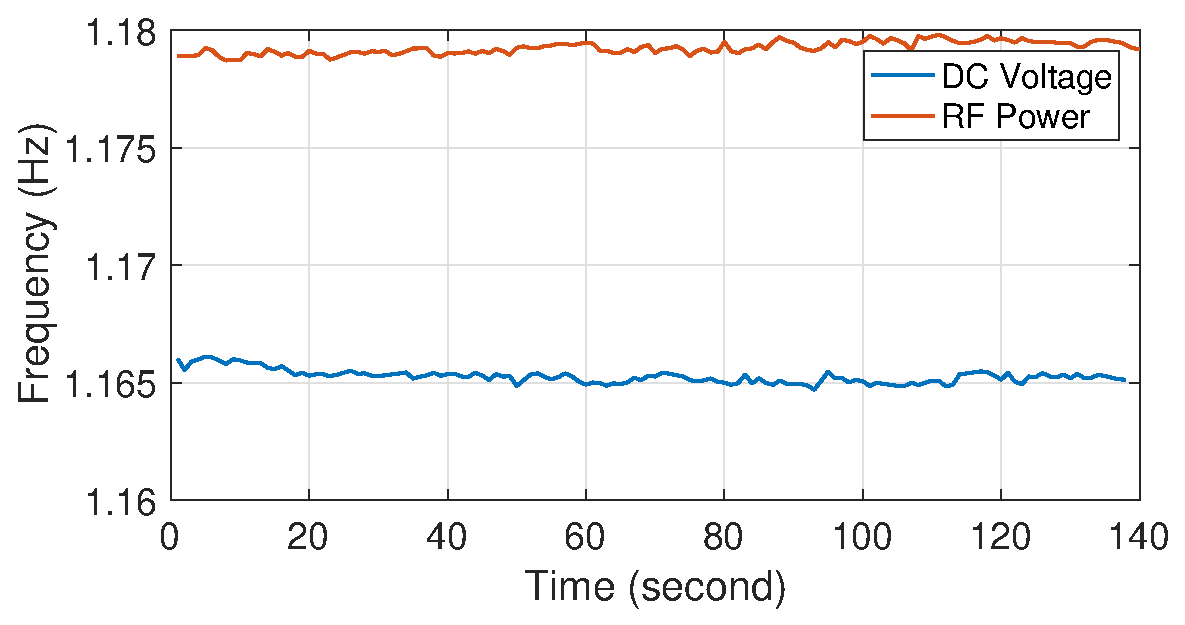
\includegraphics[width=0.85\columnwidth]{figures/clock_frequency_dc_rf.eps}
	\caption{\label{fig:frequency_dc_rf} In our testbed, see Section~\ref{sec:testbed} for the details, we programmed a single WISP tag so that it toggles one of its output port whenever its 32~KHz built-in timer progresses 32000 clock ticks. In the ideal case where the crystal oscillator of the tag does not drift, the tag would toggle its output port at each 1 second, i.e. with a frequency of 1\,Hz. During our experiment under a stable environmental temperature, we connected the output port of the tag to a logic analyzer and measured the frequency of the toggle event. We plotted our measurements when the tag is powered by the Flash Emulation Tool (FET) with a stable DC power and when the tag is powered by the RFID Reader at a distance of 5~cm. We measured the mean and standard deviation of the frequency in the DC case as 1.1653 and 0.00028553, and these values for the RF case were 1.1793 and 0.00026049, respectively. }
\end{figure}

\add{\subsubsection{Slot and bit-level synchronization} EPC Gen2 requires a slot-level synchronization to implement slotted Aloha protocol. This is achieved by adjusting clock offsets upon reception from the reader and introducing guard times to ensure that tags communicate at the
allocated frame boundaries. It is also possible to exploit modulation properties of signals from the reader to the tags (such as bit timing in FM0 modulation) in order to get the timing measurements of the regular patterns in the signal, i.e. bit-level synchronization~\cite{liu_tcomp_2015,liu_ton_2017,liu2_ton_2017}. However, neither slot nor bit level synchronization compensate for clock drifts and output a synchronized clock value that can be accessed by the tags.}

\subsubsection{Continuously varying voltage level} In WSNs, the battery level decreases gradually that allows stable voltage levels in the short term. On the contrary, on the WISP platform, the fluctuating input voltage prevents short-term stability of the clock hardware and introduces significant drift. \add{Even though embedded platforms are equipped with voltage regulators, the output of these regulators also exhibit instability and inaccuracy with respect to the input voltage; i.e. they are not perfect and they have an input voltage transient response. Therefore, they have an output voltage variation with respect to the input voltage---still leading to clock frequency instabilities.} Hence, the prominent factor affecting the frequency of the crystal oscillator is the varying voltage level, see Fig.~\ref{fig:frequency_dc_rf}.

\subsubsection{Frequent power failures} Contrary to sensor nodes, WISP tags frequently ``die'' due to power loss and they need to save the synchronization state, e.g. the clock offset and relative frequency, into the non-volatile memory to recover when they harvested sufficient energy to start up. However, saving computational state is also an energy consuming task~\cite{blisp}.

\subsubsection{Energy and resource constraints} The classical motto of WSNs, ``compute instead of communicate whenever possible''~\cite[p. 44]{karl2007protocols}, is no longer valid for the WISP platform since backscatter communication comes almost for free~\cite{ekhonet}. Due to the intermittent power, lightweight methods in terms of computation and memory are required for the synchronization. Since methods like least-squares regression are computationally heavy and require considerable amount of memory~\cite{pi2015} they should be avoided. 

\subsubsection{Limitations of the EPC Gen 2 standard} The WISP firmware implements the EPC Gen 2 standard~\cite{epc_gen2} which increases the compatibility with the existing RFID systems. However, the standard introduces limitations, e.g. currently it does not assign timestamps to the radio packets, which is a fundamental requirement to establish synchronization. Moreover, communication delays between the reader and tag are quite dependent on the implementation of this standard by RFID readers. Unfortunately, these issues lead to less accurate synchronization as compared to existing WSN solutions, as shown by our measurements presented in the following sections. Consequently, WSN synchronization protocols that can guarantee $\mu s$-level synchronization accuracy, e.g.~\cite{Maroti2004}, are hard to achieve in CRFID domain.

\section{WISP Hardware and CRFID Networks: A Brief Look}
\label{sec:Clock_Hardware}

In this section we present brief information about the WISP hardware, in particular its clock system. For the sake of clarity, we 
also give details about a typical CRFID network, which we used to implement and evaluate our synchronization methods in this article.

\subsection{Low Power Operation Modes and The Clock System}
\label{subsec:clock_system}

The WISP 5.0 platform comes with the MSP430FR5969 \cite{msp430fr5969_data_sheet} microcontroller (later called as MSP430 in this article) with FRAM non-volatile memory. The MSP430 clock system includes (i) a 32\,kHz external crystal oscillator, (ii) an internal very-low-power low-frequency oscillator, and (iii) an integrated internal digitally controlled oscillator (DCO). The five built-in 16-bit timers (TA0--TA3, TB0) in this system can be clocked with the auxiliary clock (ACLK) signal that is sourced from the relatively stable external 32\,kHz oscillator. The MSP430 has one active mode and seven software selectable low-power operation modes. Low Power operation Mode 3 (LPM3) is the standby mode where CPU, FRAM and high-frequency peripherals are off; the external 32\,kHz oscillator and the ACKL signal are active. In our target implementations, we configured TB0 to be clocked  with ACKL so that it has 16-bit 32\,kHz precision and runs continuously in LPM3 mode.

\subsection{\label{sec:testbed}An Experimental CRFID System}


\begin{figure}
	\centering
	\begin{tikzpicture}
	\node[anchor=south west, inner sep=0] at 
	(0,0){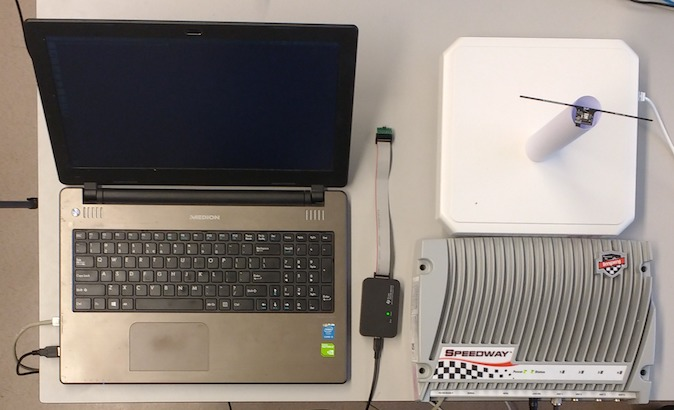
\includegraphics[width=\columnwidth]{figures/testbed_resized.jpg}};
	
	\node [fill= white,circle] at (7,2) { };
	\node [color=black ] at (7,2) { 1 };
	
	\node [fill= white,circle] at (8,4) {  };
	\node [color=black ] at (8,4) { 2 };
	
	\node [fill= white,circle] at (4,2) {  };
	\node [color=black ] at (4,2) { 3 };
	
	\node [fill= white,circle] at (5.1,2) {  };
	\node [color=black ] at (5.1,2) { 4 };
	
	\node [fill= white,circle] at (6.5,4.5) {  };
	\node [color=black ] at (6.5,4.5) { 5 };
	
	\end{tikzpicture}
	\caption{\label{fig:crfid_testbed} A single-hop CRFID testbed: (1) an Impinj Speedway R1000 RFID reader, (2) a single WISP 5.1 tag, (3) a host computer, (4) FET programmer and (5) a Laird S9028PCR antenna. The same testbed setup has been used previously in~\cite{wisent:2016} by us to evaluate downstream data transmission in CRFIDs.}
\end{figure}

As presented in Fig.~\ref{fig:crfid_testbed}, a typical CRFID system is composed of an RFID reader, a single WISP tag placed inside the communication range of this reader and a host computer to control this reader. In our testbed, we used a 915\,MHz Impinj Speedway R1000 RFID reader with firmware version 3.2.4 connected to a Laird S9028PCR 8.5\,dBic gain antenna. We placed the WISP tag at the line-of-sight from the reader antenna. For the host-reader control operations, we used sllurp~\cite{sllrp_github}, a LLRP (Low-Level Reader Protocol)~\cite{llrp}  control library written in Python.  To program the WISP tag, we used MSP430 Flash Emulation Tool (FET), in combination with TI Code Composer Studio (CCS), attached to the host.  All of our experimental evaluation presented in the next sections were conducted using this setup at a university office with human presence.

\subsection{\label{sec:sniffer}A Sniffer for the CRFID System}


Communication delays are one of the main sources of errors in synchronization~\cite{Maroti2004} and they should be kept as small as possible. In order to characterize the communication delays between the RFID reader and the WISP tags during backscatter communication and understand the effect of these delays on the synchronization error, we used USRP 210 software-defined radio, another Laird antenna placed at 50\,cm from the tag and the GNU Radio toolkit~\cite{gnuradio} with the custom software to sniff the radio packets. The sniffer was presented first in~\cite{stork:2017} and we refer the reader to this study for more details. Implementing sniffing mechanism allowed us to store the timings of the transmission and reception of the EPC Gen 2 packets, which we later processed offline to measure the actual transmission delays. We will present these measurements in the next sections. 
\section{System Model, Notation and Preliminaries}
\label{sec:clock_model}

In this section, we provide a mathematical framework that models the built-in clocks and in particular the clock drifts of the WISP tags and the RFID reader. We will use these models to prove the correctness of our synchronization algorithms and to derive mathematical expressions that represent their synchronization performance.
\begin{figure*}
	\centering
	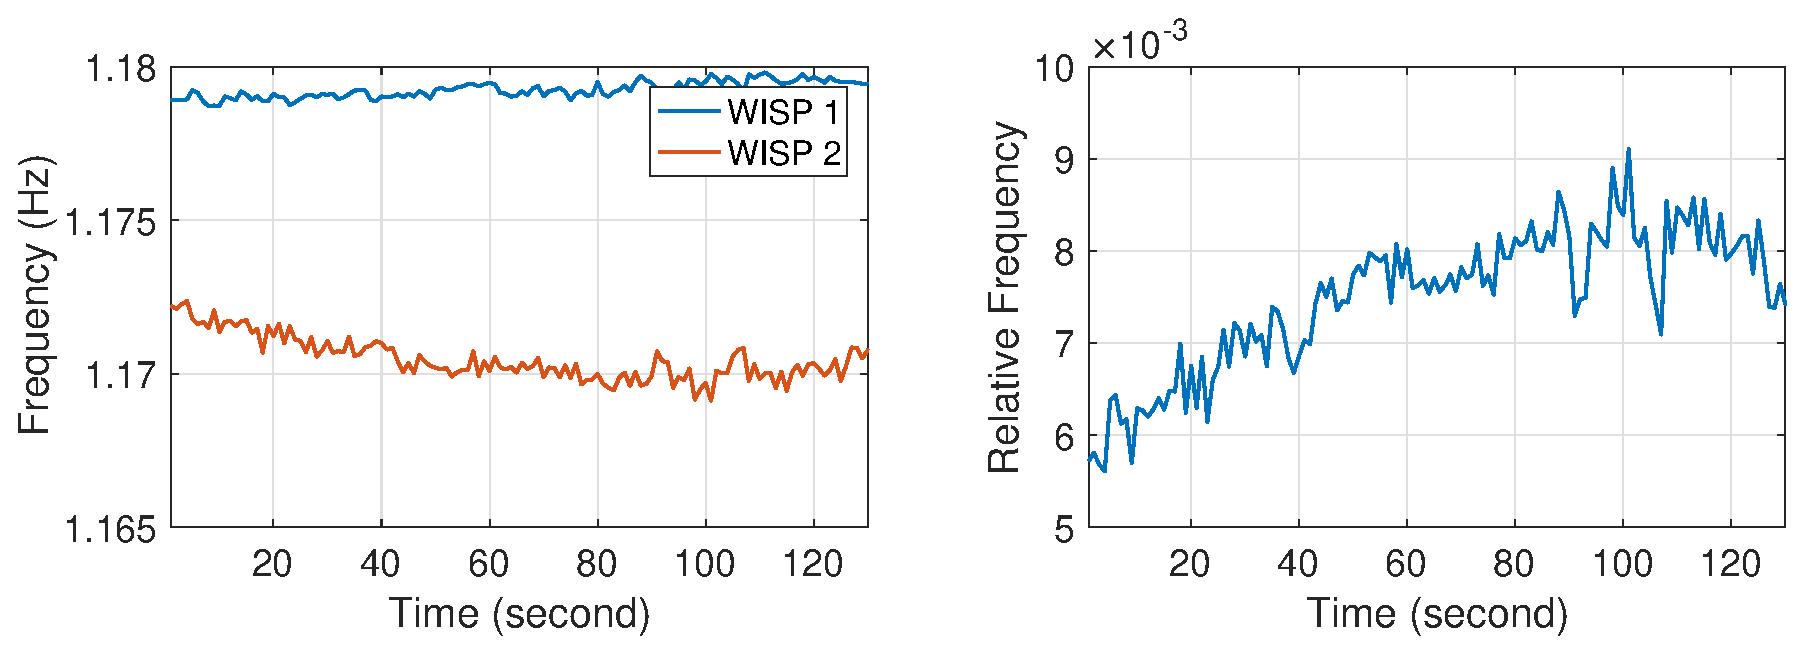
\includegraphics[width=1.4\columnwidth] {figures/relative_clock_frequency.eps}
	\caption{\label{fig:frequency}The frequencies of the toggle events (obtained using the same steps presented in Fig.\ref{fig:frequency_dc_rf}) of two RF-powered WISP tags, placed at 5 cm distance from the RFID reader. On the left the individual event frequencies ($f_1$ and $f_2$) are presented, and their relative clock frequency ($\frac{f_1}{f_2}-1$) is presented on the right. We measured the mean and standard deviation of $f_1$ as 1.1793 and 0.00026049 and those of $f_2$ as 1.1705 and  0.00068239, respectively.}
\end{figure*}
In this framework, we denote a single WISP tag by $w$ and the RFID reader by $r$. The Timer B0 mentioned in Section~\ref{subsec:clock_system} can be considered as the built-in clock, i.e. \emph{local clock}, of the tag $w$, 
which we denote by $C_{w}$. The value of $C_{w}$ at time $t$ can be modeled as
%
\begin{eqnarray}
C_{w}(t) & \triangleq & C_w(t_0)+ \int_{t_0}^{t}f_{w}(u)du, 
\label{eq:local_clock}
\end{eqnarray}
%
where $t_0$ represents the time at which tag $w$ is powered on and  $f_{w}(u)$ represents the \emph{instantaneous oscillator frequency} of $C_{w}$ at time $u$. Since the frequency of the oscillators are affected by environmental factors such as temperature and voltage level, they are not stable~\cite{Lenzen2009Optimal} and $f_{w}$ is not a constant but it is \emph{time varying}, see Fig.~\ref{fig:frequency}. From \eqref{eq:local_clock}, it can be noticed that $C_w$ is \emph{unitless}. Indeed, it can be seen as a counter of oscillation events that are produced at a frequency of $f_w$.

The RFID reader $r$ can be considered as a natural time reference for the tag $w$. We denote the local clock of the RFID reader at time $t$ by $C_{r}(t)$ and its frequency by $f_r(t)$. By collecting (time) information from the RFID reader, the tag $w$ runs a \emph{clock synchronization algorithm} to calculate a \emph{software clock}, denoted by $S_{w}(t)$, whose value represents the synchronized notion of time. The objective of the synchronization algorithm is minimizing the \emph{synchronization error} with respect to the reader $r$ at any time $t$, which is defined as 
%
\begin{eqnarray}
\gamma(t)&\triangleq&S_w(t)-C_r(t). \label{eq:gamma_error}
\end{eqnarray}
%
Considering the individual clock frequencies $f_w$ and $f_r$, we denote the \emph{instantaneous relative clock 
	frequency} of the WISP tag 
with respect to the RFID reader at time $t$ as
%
\begin{eqnarray}
f_w^r(t)&\triangleq&\frac{f_w(t)}{f_r(t)}-1. \label{eq:relative_frequency}	
\end{eqnarray}
\section{Sender-Receiver Based Reader-Tag Synchronization in CRFID Systems}
\label{sec:sender_receiver}

In this section we provide initial observations, design and implementation of a \emph{sender-receiver} based synchronization approach that synchronizes a single WISP tag to the RFID reader and we reveal its limitations in current CRFID networks. In sender-receiver based synchronization mechanisms, receiver devices synchronize to the clock of a reference sender device. In order to synchronize itself to the RFID reader with such a mechanism, the WISP tag should obtain several $(C_w(t),C_r(t))$ synchronization points to establish a \emph{relationship} between its local clock $C_w$ and the reader clock $C_r $, represented by its software clock $S_w$. The value $S_w(t)$ will provide an estimate of the reference clock $C_r(t)$ at any time instant $t$.

\begin{figure}
	\centering
	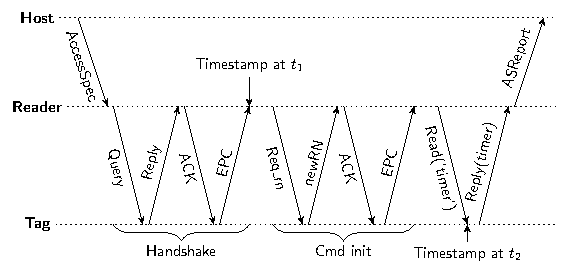
\includegraphics[width=\columnwidth]{figures/Sender-Receiver.pdf}
	\caption{\label{fig:sender_receiver} The message exchange among the host computer, the RFID reader and the tag for sender-receiver synchronization. The host machine, i.e. a PC,  sends the high level commands to the reader via LLRP \emph{AccessSpec} message and receives the results through an \emph{ASReport}. The RFID reader follows the steps defined in the EPC Gen2 standard: (i) performs a \emph{Handshake} to initialize the communication with the active tag; (ii) performs a \emph{Command Initialization} (Cmd Init) by requesting a random number from the tag (Req\_n) and receiving the random number (newRN); (iii)  performs a \emph{Read} command by sending its request and receiving the timer value. The reader assigns the \emph{FirstSeenTimestamp} to the tag at time $t_1$ and the tag timestamps the command reception event at time $t_2$ with its local clock reading.}
\end{figure}

We explored the EPC Gen2 standard and the LLRP protocol and found out that LLRP assigns a \emph{FirstSeenTimestamp} in UTC (Coordinated Universal Time), which is defined as \emph{``The Reader SHALL set it to the time of the first observation amongst the tag reports that get accumulated in the TagReportData''} \cite[p. 87]{llrp}. From this definition, we assume that this timestamp is assigned by the reader when it receives the EPC during the handshake operation with the corresponding tag, shown in Fig. \ref{fig:sender_receiver} as the timestamp assigned at time $t_1$. Therefore, the \emph{FirstSeenTimestamp} can be considered as $C_r(t_1)$. In order to obtain the corresponding local time $C_w(t_1)$, one strategy is to force the reader to send a special ``synchronization'' command after the handshake so that the tag timestamps the command reception event using its local clock, shown in Fig.\,\ref{fig:sender_receiver} as time $t_2$. As we emphasized in Section~\ref{sec:WSN-Sync}, transmission delays are the main source of errors in time synchronization and they should be kept as deterministic as possible. We denote the \emph{transmission delay} in this case by $\Delta t= t_2-t_1$ and it is desirable to keep the \emph{variation} of $\Delta t$, i.e. \emph{jitter}, as small as possible~\cite{Maroti2004}.

\subsection{Transmission Delay and Jitter Measurements}

\begin{figure}
	\centering
	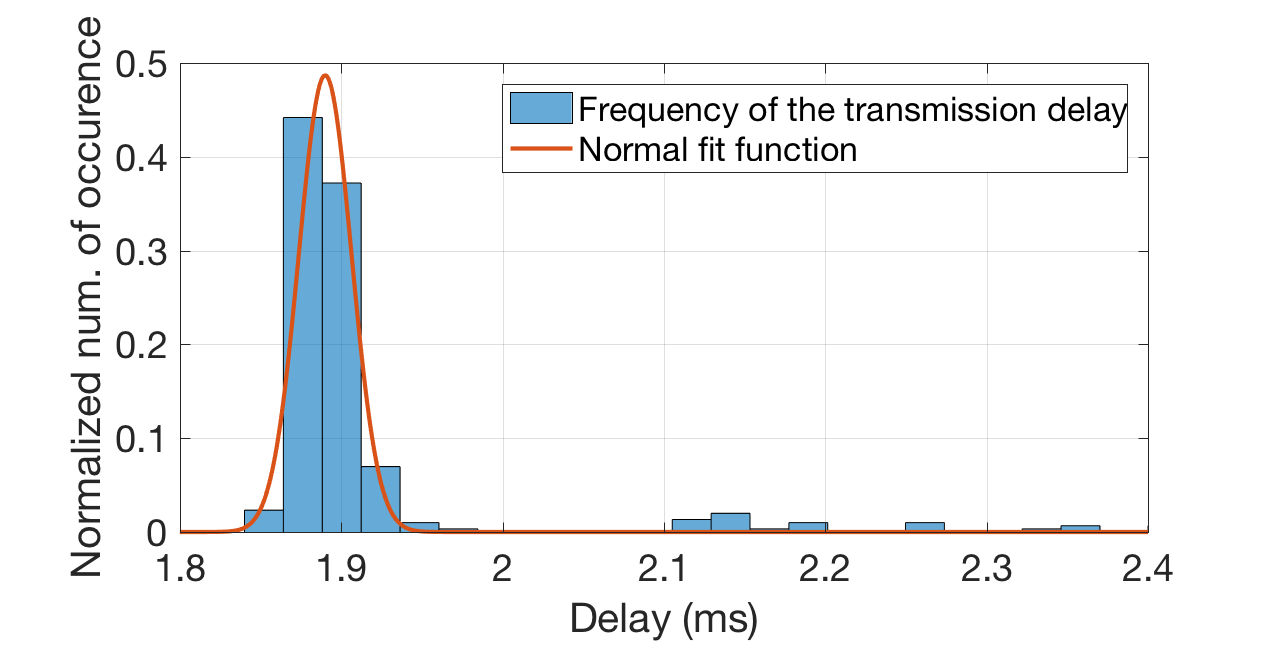
\includegraphics[width=0.9\columnwidth]{figures/sender_receiver_uncertainty.eps}
	\caption{\label{fig:transmission_delay} The normalized number of occurrences of the transmission delays measured by sniffing the communication between the RFID reader and the WISP tag. We calculated the mean transmission delay and its standard deviation as 1.89\,ms and 0.0164\,ms with a 99\% confidence interval of [1.8874,1.8925] and [0.0148,0.0184], respectively.}
\end{figure}

In order to characterize the transmission delay $\Delta t$, we placed the WISP tag 20 cm away from the antenna using the setup presented in Fig.~\ref{fig:crfid_testbed} and we sniffed the communication between the RFID reader and the WISP tag during the communication scenario of Fig.~\ref{fig:sender_receiver}. Fig.~\ref{fig:transmission_delay} presents a summary of our measurements (with 300 samples gathered). We observed that the transmission delay is distributed with a mean of 1.89\,ms and standard deviation of 0.0164\,ms. Moreover, we observed some outliers, presented at the right hand side of the figure, which we attribute to the EPC Gen2 implementation of the Impinj reader. 

\subsection{Collection of Clock Values for Off-line Processing}

After characterizing the variation of the transmission delay, the next step was the collection of the clock values from the RFID Reader and the WISP tag in order to try synchronization mechanisms offline, which allowed to evaluate the performance of sender-receiver synchronization mechanism in CRFID networks. We collected $(C_w(t_2),C_r(t_1))$ pairs for offline processing by controlling the RFID reader to send a \emph{Read} command to the tag and by programming the WISP tag so that it backscatters $C_w(t_2)$ upon receiving this command. The received pairs $(C_w(t_2),C_r(t_1))$ were logged by the host computer. 

\subsection{Software Clock Computation Using  Least-Squares}

Following studies~\cite{Maroti2004,Schmid:2010,Lenzen:2015,TATS:2016} that use a linear clock model, we assume a \emph{linear} relationship between $C_r$ and $C_w$ and we model the software clock of the WISP tag as $S_w(C_w(t)) = a + b C_w(t)$ where $S_w$ represents an estimator of the reader's clock $C_r$, $a$ is the \emph{offset} and $b$ is the \emph{relative speed} with respect to the local clock $C_w$. To establish such a relationship, we performed \emph{least-squares regression} offline in MATLAB using the collected pairs in the previous subsection. As in \cite{Maroti2004}, since the WISP tag has limited memory, computation capability and energy, at each step only the most recent $N$ pairs are used to estimate the regression line. 

\begin{figure}
	\centering
	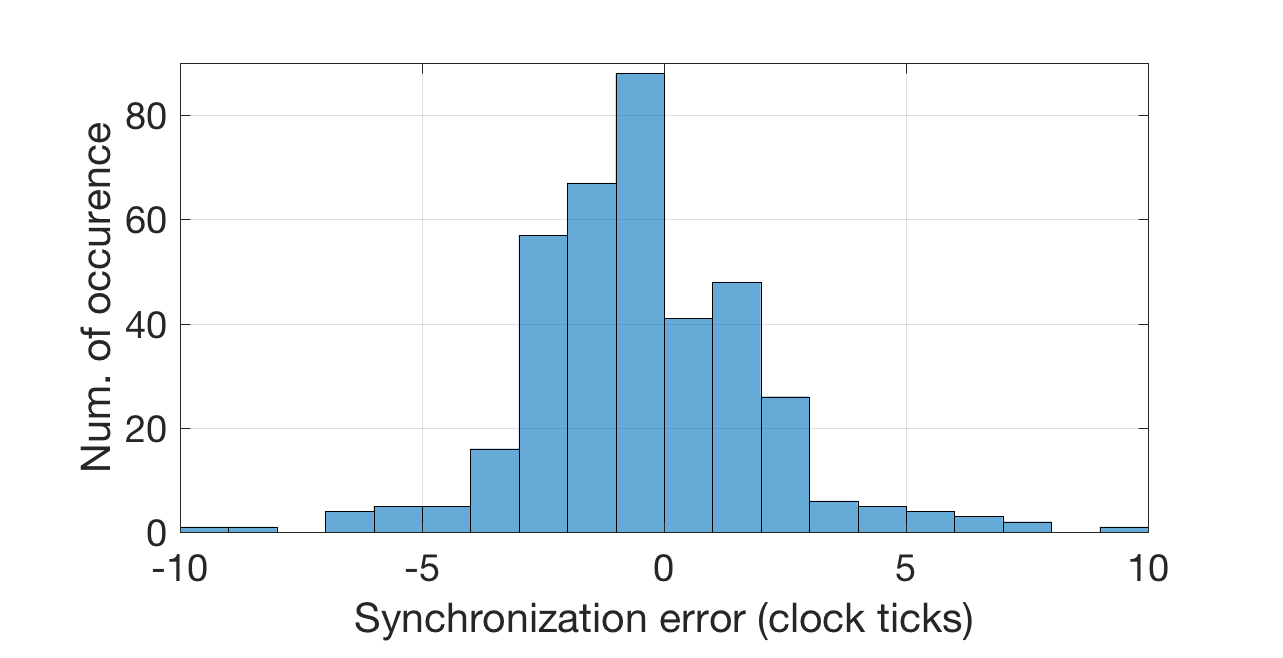
\includegraphics[width=0.9\columnwidth]{figures/least_squares.eps}
	\caption{\label{fig:least-squares}Synchronization error by employing least-squares regression on the collected timestamps. We observed a maximum synchronization error of 10 clock ticks between the RFID reader and the WISP tag, leading to 0.32\,ms synchronization accuracy.}
\end{figure}

Formally, let $[C_w(t_k),C_r(t_k)]$ denote the $k$th pair in the log file where $t_k$ denotes the real-time at which 
\emph{FirstSeenTimestamp} has been assigned during the collection of this pair. At each $k$th step, the pairs $\{[C_w(t_k),C_r(t_k)],$\ldots$,[(C_w(t_{k+N-1}),C_r(t_{k+N-1})]\}$ are used to calculate the parameters $a$ and $b$, i.e. the \emph{intercept} and the \emph{slope} of the estimated regression line \cite{book-SheldonRoss}, using \textsf{polyfit} function of MATLAB. We calculated the synchronization error as 
$\gamma(t_{k+N})\triangleq S_w(C_w(t_{k+N}))-C_r(t_{k+N})$
%
that represents the difference between the predicted reference time and the received reference time. In our implementation we used $N=8$ as in~\cite{Maroti2004} and Fig.~\ref{fig:least-squares} presents the synchronization error at each step. We observed a maximum synchronization error of 0.32\,ms in this one-hop network, which is more than one order of magnitude larger than the synchronization performance of the de facto WSN solution \cite{Maroti2004}, which was reported as approximately 10\,$\mu$s.

\subsection{Limitations of the Approach}

In addition to the challenges listed in Section \ref{sec:CRFIDs}, we observed two crucial limitations for the WISP platform, which prevents to build up a sender-receiver synchronization building block:

\subsubsection{Host computer computation} We are unaware of any EPC Gen2 command that will allow to send the \emph{FistSeenTimestamp} to the tag. Hence, even though we were able to collect $(C_w(t),C_r(t))$ pairs for offline processing, it is not possible for the tag to collect $C_r(t)$ and synchronize itself to the reader. Therefore, with this limitation, only a host computer can collect and log the timestamps, calculate the relationship between the clock of the tag and the clock of the reader and send the data that represents this relationship to the tag for synchronization, making this method only of theoretical nature as of now. 

\subsubsection{The Lack of broadcast primitive} Since the RFID reader assigns the \emph{FirstSeenTimestamp} for each tag, the synchronization steps in Fig.~\ref{fig:sender_receiver} should be repeated for each tag to obtain synchronization in the communication domain of the reader. 
%Unfortunately, in the current EPC Gen2 and LLRP standard, we were unable to find any mechanism to send a global timestamp that is received by all tags inside the range of the RFID reader to establish synchronization in one step.

\subsubsection{Big and reader dependent transmission delays} As depicted previously, we observed that transmission delays in our testbed were on the order of milliseconds, see Fig.~\ref{fig:least-squares}, whereas they are reported as a few microseconds in conventional WSN platforms. This is one of the crucial limitations since the smaller the transmission delays are, the better the synchronization.

\section{Event-Based Reader-Tag Synchronization In CRFID Systems}\label{sec:event_based}

In this section, we introduce a simple but novel \emph{event-based} reader-tag synchronization inspired by simple PI controllers and provide its advantages over the previous approach. In event-based synchronization, a common event which is observable by all receiver devices simultaneously is generated by the reference device. Upon receiving events generated at regular intervals, receiver devices can predict the occurrence time of future events. In order to synchronize the tag with such a mechanism, the RFID reader does not send explicit timestamp values as in sender-receiver based synchronization but instead generates events at regular intervals. Upon observing these events, the receiver tag adjusts the rate of its software clock so that it predicts the occurrence of the next event precisely. 
\begin{figure}
	\centering
	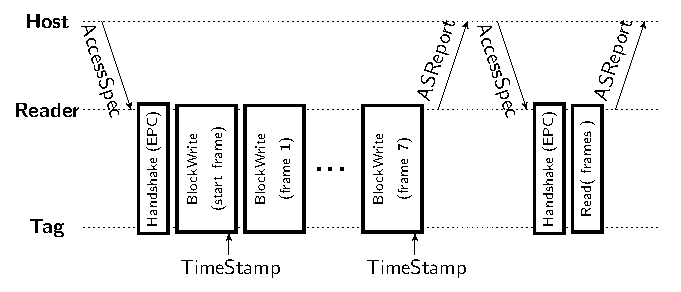
\includegraphics[width=\columnwidth]{figures/Event-Based.pdf}
	\caption{\label{fig:event_based}Event-Based synchronization steps: The tag timestamps successive \emph{BlockWrite} events and adjusts its software clock.}
\end{figure}
We explored the EPC Gen2 standard to see how to generate events at regular intervals and realized that the \emph{BlockWrite} operation allows this feature.\footnote{It is possible to exploit modulation properties of signals from the reader to tags (such as bit timing in FM0, i.e. Miller 1, modulation) in order to get the timing measurements of the regular patterns in the signal. However, this requires using a high-precision clock to obtain microsecond-precision timing measurements. In this study, we used the higher-level properties of the EPC Gen2 standard, rather than exploiting its low-level signal properties. By means of this, we could  use the external 32\,KHz clock that runs even in low-power standby mode (see Section \ref{sec:Clock_Hardware}) to obtain timing measurements.)} Fig.~\ref{fig:event_based} presents the steps of event-based synchronization. During the command phase, the EPC Gen2 standard allows a maximum of eight successive \emph{BlockWrite} operations. It is desirable to use the first and the last \emph{BlockWrite} events for synchronization since it is better to compensate frequency differences observed in longer time intervals to adjust the software clock. 

\subsection{Event Period Measurements}
\label{subsec:event_period_uncertainty}

\begin{figure}
	\centering
	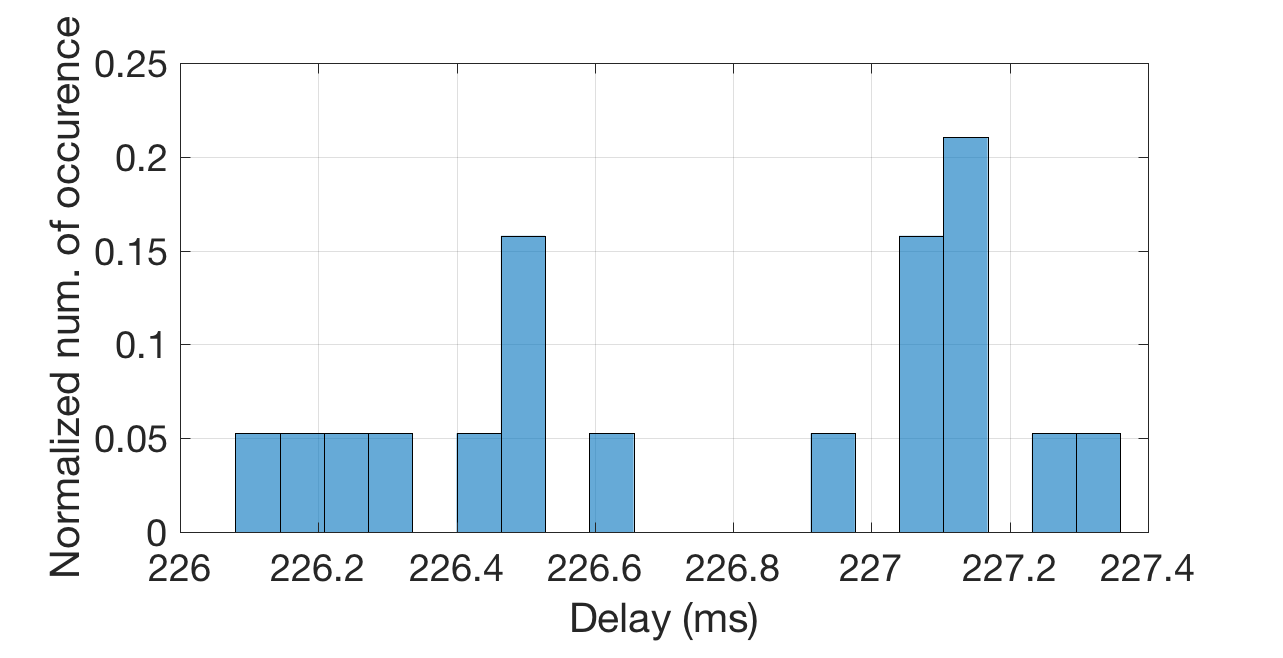
\includegraphics[width = 0.9\columnwidth]{figures/blockwrite_delay.eps}
	\caption{\label{fig:block_write_delay}The delay between the first and the last \emph{BlockWrite} event, i.e. \emph{event period}, by considering 20 samples during the communication scenario in Fig.~\ref{fig:event_based}. We measured its mean and standard deviation as 226.7667\,ms and 0.4097\,ms with a 99\% confidence interval of [226.4961,227.0372] and [0.2852,0.6945], respectively.}
\end{figure}

The real-time length between the first and the last \emph{BlockWrite} operation is the \emph{event period}, we denote by $\tau$, and its variation is the main error source. Therefore, it is important to explore its characteristics. We sniffed the communication protocol between the RFID reader and a tag presented in Fig. \ref{fig:event_based}. We took 20 sample measurements about the \emph{event period}, which is summarized in Fig.~\ref{fig:block_write_delay}. According to our measurements, the \emph{event period} was distributed with a mean of 226.76\,ms and standard deviation of 0.41\,ms; respectively. We would like to mention that these values are dependent on the RFID Reader implementation of the EPC Gen2 protocol.

\subsection{Event-Based Synchronization Inspired By PI Controllers}

For the computation of the software clock, \emph{adaptive} and \emph{lightweight} solutions are crucial due to the following important requirements:

\begin{itemize}
	\item Since the voltage level is not stable and the harvested power is limited, the computations should demand little amount of energy to calculate the software clock, i.e. marginal number of steps---\emph{Addressing Challenge I in Section~\ref{sec:Motivation}}.
	
	\item Since power is intermittent, the number of variables pertaining to the software clock should be marginal so that saving the state of the synchronization to non-volatile memory will demand little time and less energy. Therefore, lightweight computation methods in terms of main memory overhead are required---\emph{Addressing Challenge I in Section~\ref{sec:Motivation}}.
	
	\item Unstable voltage level leads to frequently varying clock frequencies. Therefore, the computation methods should adapt such dynamic conditions in a very fast manner to keep synchronization accuracy stable---\emph{Addressing Challenge II in Section~\ref{sec:Motivation}}
\end{itemize}

Considering these facts, we designed a lightweight and adaptive clock synchronization approach inspired by the PI-controller based solution introduced in~\cite{pi2015,yildirim2017adaptive}: (i) we apply PI-controller based clock computation technique to the WISP platform due to its computational efficiency and fast adaptation; (ii) we introduce power-interrupt recovery mechanism so that the WISP tags do not loose their synchronization-related information. We modified the algorithm in our previous work so that PI-controllers use the periodic event occurrences rather than explicit clock values of a master node. We also provide a moderately different but more realistic theoretical analysis by using a more realistic clock drift model, i.e. Brownian motion rather than uniform distribution---see Appendix.

Let $t_0$ denote the first event reception time at the tag. Using the pre-measured event period $\tau$ of the RFID reader, the tag can estimate the next event reception time at time $t_1$ as
\begin{eqnarray}
\hat{C}_w(t_1) &=& C_w(t_0)+\tau(1+\hat{f}_w^r(t_0)), \label{eq:core}
\end{eqnarray}
where $\hat{f}_w^r(t_0)$ denotes the \emph{estimated relative frequency} at time $t_0$, which is an estimate for \eqref{eq:relative_frequency}. The intuition behind \eqref{eq:core} is that $1+\hat{f}_w^r(t_0)$ gives the estimated value of $f_r(t_0)/f_w(t_0)$, $\tau f_r(t_0)$ gives the estimated local time passed on the reader side and $\tau f_r(t_0)/f_w(t_0)$ gives the estimated number of clock ticks on the tag side that will pass until the next packet reception. Redefining \eqref{eq:gamma_error}, the \emph{prediction error} at time $t_1$ can be written as
\begin{eqnarray}
\gamma(t_1) & \!\!\!\!\!=\!\!\!\!\!\! & 
C_{w}(t_{1}\!)\!-\!\hat{C}_{w}(t_{1}\!) \!=\! 
C_{w}(t_{1}\!)\!-\!C_{w}(t_{0}\!)\!-\!\tau(1\!\!+\!\!\hat{f}_{w}^{r}(t_0\!)). \label{eq:gamma_t_1}
\end{eqnarray}
Apparently, the objective is to minimize the prediction error so that the event reception time is estimated correctly. As can be observed from \eqref{eq:gamma_t_1}, the estimation error on the relative clock frequency at time $t_0$, i.e. $\hat{f}_w^r(t_0)$, depends on the mean event period $\tau$, and its variance (since they affect $C_w(t_1)-C_w(t_0)$). Inspired by the integral controller update rule in \cite[Section III, (5)]{pi2015}, we propose to update the estimated relative frequency at time $t_1$ as
\begin{eqnarray}
\hat{f}_{w}^{r}(t_1) &=& \hat{f}_{w}^{r}(t_0)+\beta\gamma(t_1), 
\label{eq:update_rule}
\end{eqnarray}
where $\beta$ is the \emph{integral gain}. Assume that the uncertainty of the event period is $\varepsilon\sim\mathcal{N}(0,\sigma^2_{\tau})$ and the instantaneous change on the relative clock frequency is $\frac{df_{w}^{r}(t)}{dt}\sim\mathcal{N}(0,\sigma_{\eta}^{2})$. Under these assumptions, it can be proven that if $0<\beta<\frac{2}{\tau}$ is satisfied the synchronization will hold eventually; i.e. $\hat{f}_{w}^{r}=f_{w}^{r}$. Moreover, the mean and the variance ($\sigma^2_\gamma$) of the steady-state (asymptotic) estimation error of WISP-Sync can be given by 
\begin{eqnarray}
\gamma & \!\!\!\!\!\sim\!\!\!\!\! & \mathcal{N} \!\!\left(\!\!0,\sigma^2_\gamma\!\!=\!\!\frac{\sigma^2_{\eta}\!\left(\!\tau^2\!-\!\beta\tau^3\!+\!\frac{\beta^2\tau^4}{3}\!\right)\!\!+\!\!\beta^2\sigma^2_{\tau}\tau}{(2\beta-\beta^2\tau)}\!\!+\!\!\frac{\sigma^2_{\eta}\tau^3}{3}\!+\!\sigma^2_{\tau} \!\!\right),
\label{eq:sync_performance}
\end{eqnarray}
which is derived in Section~\ref{sec:app_b} of the Appendix.

\begin{figure}
	\centering
	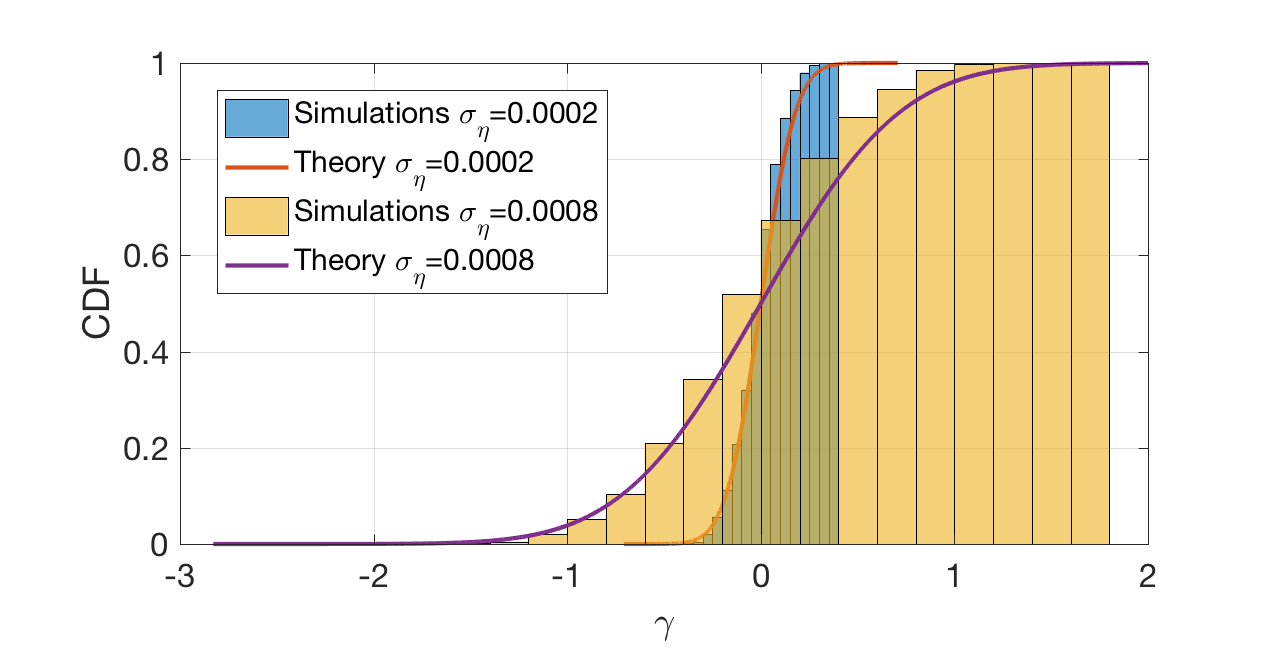
\includegraphics[width=\columnwidth]{figures/sim-theory.eps}
	\caption{\label{fig:theory-vs-simulations} The plot of the cumulative distribution function (CDF) of $\gamma$ in \eqref{eq:sync_performance} and the CDF of the steady-state $\gamma$ obtained during numerical simulations of \eqref{eq:update_rule} (by implementing \eqref{eq:theta} and \eqref{eq:delta_recursive} in Appendix). We used $\tau=1$, $\beta= 0.0001$, $\sigma_{\tau}=0.00005$ and our plots depict the theoretical and simulation results with respect to $\sigma_\eta = 0.0002$ and $\sigma_\eta = 0.0008.$ It can be observed that \eqref{eq:sync_performance} is consistent with the simulations and bigger uncertainty leads to bigger synchronization error.}
\end{figure}
In Fig.~\ref{fig:theory-vs-simulations}, we emphasize that our theoretical derivation in \eqref{eq:sync_performance} is consistent with the simulations of \eqref{eq:update_rule}. We refer again the reader to the Appendix for the detailed proofs of the convergence and the asymptotic estimation error. Moreover, in Section~\ref{sec:adaptibility}, we discuss the impact of the parameters $\tau$ and $\beta$ on the synchronization accuracy.

\subsubsection{The Synchronization Algorithm}

\begin{algorithm}[t]
%	\setstretch{1.35}
	\caption{\label{alg:sync} \emph{WISP-Sync}: An integral controller-based 
		algorithm at WISP tag side.}
	\begin{algorithmic}[1]	
		\small	
		
		\Statex\textbf{Definitions:}
		\Statex$t_f$ \Comment{local time of the first \emph{BlockWrite}} 
		\Statex $C_w$ \Comment{bult-in clock of the WISP tag}
		\Statex $\hat{f}_w^r\leftarrow0$ \Comment{estimated relative clock 
			frequency}	
		\Statex $\tau\leftarrow$measured value \Comment{mean \emph{event period}}	
		\Statex $\beta\leftarrow$ a value satisfying 
		$0<\beta<\frac{2}{\tau}$ \Comment{integral gain}	
		\Statex $V_{\min}, V_{\text{op}}$ \Comment{voltage thresholds ($V_{\text{op}}>V_{\min}$)}
		\Statex $V_{\text{cur}}$ \Comment{current voltage}
		
		\State $\square$ \textbf{Upon receiving the first \emph{BlockWrite}} 
		\State \quad $ t_f = C_w$ \Comment{store the local time in $t_f$}
		\State $\square$ \textbf{Upon receiving the last \emph{BlockWrite}} 
		\State \quad $\gamma = C_w- (t_f+\tau(1+\hat{f}_w^r))$ 
		\Comment{calculate estimation error $\gamma$} 
		\State \quad $\hat{f}_w^r = \hat{f}_w^r +\beta\gamma$ \Comment{apply 
			integral control}
		\State $\square$ \textbf{Upon} $V_{\text{cur}}=V_{\min}$
		\State \quad store $\hat{f}_w^r$ into FRAM \Comment{store in non-volatile memory}
		\State $\square$ \textbf{Upon} $V_{\text{cur}} < V_{\text{op}}$
		\State \quad restore $\hat{f}_w^r$ from FRAM \Comment{restore the clock frequency}
	\end{algorithmic}	
\end{algorithm}

Based on this model we introduce Algorithm \ref{alg:sync}, namely \emph{WISP-Sync}, that synchronizes the speed of the software clock to the reference clock's speed using the update rule defined in \eqref{eq:update_rule}. The steps of this algorithm can be explained as follows. Initially, the tag lets its software clock run at the same speed of its local clock by setting its relative clock rate to zero. Upon receiving the first \emph{BlockWrite} event (Line 1), the tag stores its local clock value at the variable $t_f$ (Line 2). After receiving the last \emph{BlockWrite} event (Line 3), first it calculates the estimation error (Line 4). Then, it applies the correction on its estimated relative rate $\hat{f}_w^r$ by multiplying the estimation error with the integral gain $\beta$ and adding it to $\hat{f}_w^r$ (Line 5). After receiving successive events, $\hat{f}_w^r$ will converge to its desired value eventually, as proven in the Appendix. 

\subsubsection{State Recovery}

Due to intermittent RF power, the tag is subject to frequent power losses, which will lead to loss of the synchronization state. In voltage-aware systems~\cite{Buettner:2011:Dewdrop,Ransford:2011:Mementos,Lucia:2015:Execution,Colin:2016:Debugger}, the general idea is to save the system state when the input voltage is below a pre-defined threshold $V_{\min}$ and then recover it back when the input voltage is above a pre-defined threshold $V_{\text{op}}$. As shown in Algorithm~\ref{alg:sync}, the only part of the system state pertaining to synchronization is the variable $\hat{f}_w^r$. Therefore, if this variable is also saved to FRAM (when there is a power loss and recovered when there is sufficient voltage) the synchronization will resume from the point of power loss, that will prevent loss of synchronization and lead to improved synchronization accuracy. These steps are summarized in Lines 6--9 of Algorithm~\ref{alg:sync}. It should be noted that these steps require hardware support so that the voltage level is monitored continuously and the corresponding voltage level indicator events are generated. Another approach can be keeping $\hat{f}_w^r$ in non-volatile memory as a \emph{persistent variable} so that the corresponding FRAM memory location of $\hat{f}_w^r$ is updated immediately when this variable is updated---eliminating the need for Lines 6--9 of Algorithm~\ref{alg:sync}, and in turn extra voltage measurement hardware, but introducing more FRAM access overhead.

\subsubsection{Computation Complexity\label{subsec:complexity}}

It can be observed that WISP-Sync employs only very simple arithmetic operations at each step, e.g. Lines 3--5 are composed of only two subtraction, two addition and two multiplication operations. Moreover, the \emph{state of synchronization}, i.e. the parameters that are required to be saved in the non-volatile memory, is represented by only the variable $\hat{f}_w^r$. As a consequence, WISP-Sync addresses \emph{Challenge I} in Section~\ref{sec:Motivation} in terms of computation and memory overhead. 

\subsubsection{Adaptability} 
\label{sec:adaptibility}

\begin{figure*}
	\centering
	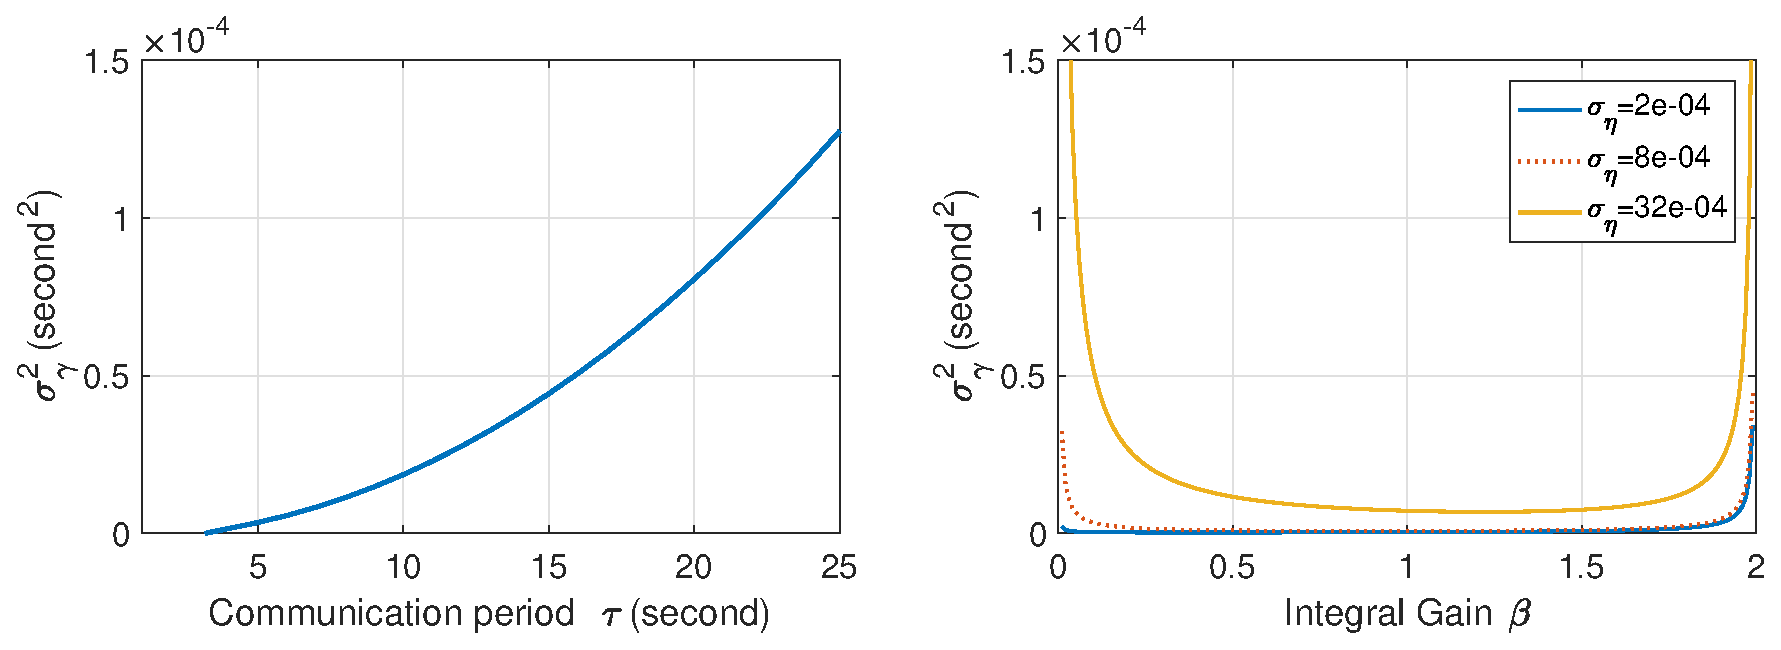
\includegraphics[width=1.4\columnwidth]{figures/alpha-period-vs-variance.eps}
	\caption{\label{fig:simulations} Numerical results showing the relations between event period, integral gain and the steady-state variance. First, we set $\sigma_{\tau}=0.4097$, $\sigma_\eta = 0.0008$, $\beta=1$ and plotted $\sigma^2_{\gamma}$ using different $\tau$ (left hand side). Observe that increasing $\tau$ increases $\sigma^2_{\gamma}$. Then, we set $\sigma_{\tau}=0.4097$,	$\tau=1$ and $\beta \in (0,2)$ due to \eqref{eq:step_size_bounds-pi}. Using different values for $\sigma_\eta$, we plotted how $\sigma^2_{\gamma}$ changes with respect to the $\beta$ (right hand side). Observe that for each value of $\sigma_\eta$, there is a particular $\beta$ that minimizes $\sigma^2_{\gamma}$.}
\end{figure*}

In Section \ref{subsec:event_period_uncertainty} we presented our measurements pertaining to the event period and showed 
that $\sigma_{\tau}=0.4097$. Moreover, from Fig.~\ref{fig:frequency}, we calculated $\sigma_{\eta} \approxeq 0.0008$ using the \textsf{normfit} function of MATLAB.  Substituting these values in \eqref{eq:sync_performance}, we performed MATLAB simulations to calculate $\sigma^2_\gamma$, which are depicted in Fig.~\ref{fig:simulations}. These simulations led us to reveal the following points:

\begin{itemize}
	\item Considering our previous measurements, it is apparent that $\sigma^2_{\tau}$ is the dominant factor effecting the synchronization performance. Therefore, it is desirable to keep transmission delay variations and also $\tau$, as small as possible. Apparently, the bigger the resynchronization period $\tau$, the worse the synchronization error is (see left hand side of Fig.~\ref{fig:simulations}). 
	
	\item Parameter $\beta$ has significant impact on the performance of the WISP-Sync. From 	\eqref{eq:sync_performance}, it can be concluded that the synchronization error can be minimized using a proper value of $\beta$. However, the $\beta$ value that minimizes 	\eqref{eq:sync_performance} depends on the parameters $\sigma_{\eta}$ and $\sigma_{\tau}$ which represent randomness of the system. In Fig.~\ref{fig:simulations} (right hand side), we fixed $\tau$ and $\sigma_{\tau}$, we used different values of $\sigma_{\eta}$ and we plotted $\sigma^2_{\gamma}$ with respect to the values of the $\beta$ that will lead to convergence. Observe that a different $\beta$ value minimizes $\sigma^2_{\gamma}$ for each different $\sigma_{\eta}$. 
	
	\item Due to varying RF power levels, $\sigma_{\eta}$ is also a time-varying value. Therefore, $\beta$ should be selected to compensate for also \emph{dynamic} $\sigma_{\eta}$ in a \emph{fast manner} to keep synchronization error within desired bounds---which addresses \emph{Challenge II} in Section~\ref{sec:Motivation}. However, the $\beta$ that minimizes $\sigma^2_{\gamma}$ may lead to longer convergence time (see Appendix). Therefore, $\beta$ also defines how \emph{reactive} WISP-Sync is against the dynamic environment, i.e. the \emph{adaptivity}.
\end{itemize}

\section{Evaluation of WISP-Sync}
\label{sec:eval-wispsync}

In order to evaluate WISP-Sync, we considered the value of $\gamma$ in Algorithm~\ref{alg:sync} (the estimation error) as an evaluation metric. We collected the local clock readings of the tag at the first and last \emph{BlockWrite} events using our testbed setup and sniffer, and used MATLAB to implement WISP-Sync algorithm which processes the collected clock values to output the software clock. This gave us the flexibility to try different approaches without reprogramming the tag.

\subsection{Selection of the Integral Gain $\beta$} 

\begin{figure}
	\centering
	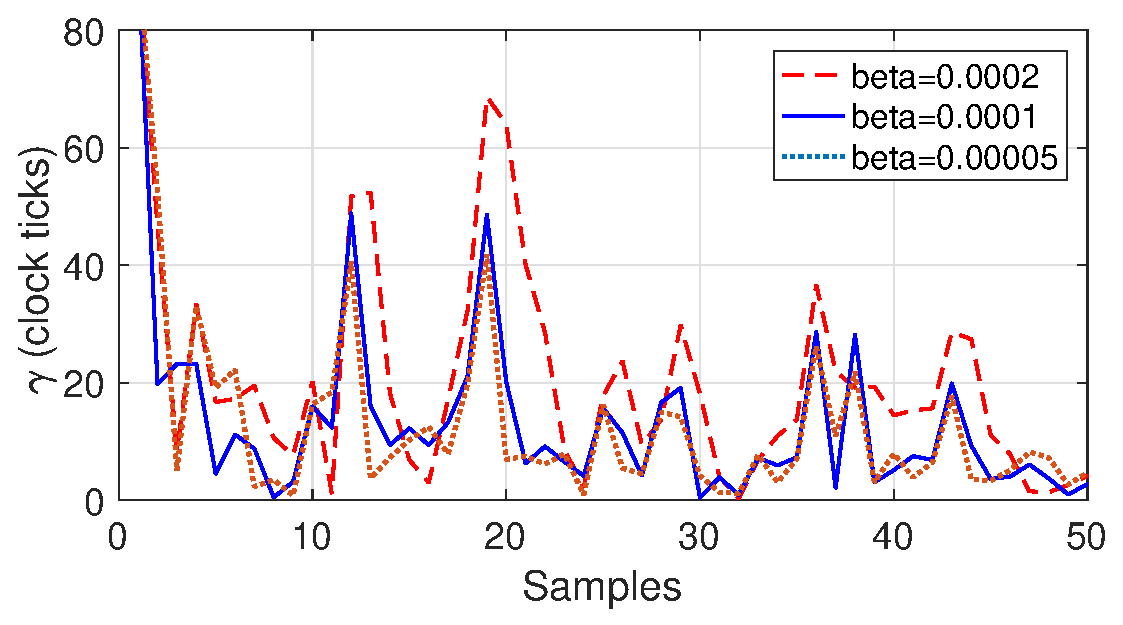
\includegraphics[width=0.85\columnwidth]{figures/integral_gain.eps}
	\caption{\label{fig:beta} The synchronization error tends to get smaller with smaller integral gains, but after some point decreasing it has no significant effect due to the precision of 32\,kHz clock. Hence, we selected a fixed value of $\beta=0.0001$ for the next steps. }
\end{figure}

Since we measured the event period as 226.76\,ms on average (see Fig.~\ref{fig:block_write_delay}), we set $\tau=7086$ 
clock ticks since the local clock of the tag is operating at 32\,kHz and each clock tick occurs every 32 microseconds. First, we explored how $\beta$ affects the performance of the algorithm. By substituting $\tau$ into \eqref{eq:step_size_bounds-pi}, the convergence condition becomes $0<\beta<0.000284$ in our case. We present the synchronization error with different $\beta$ values in Fig.~\ref{fig:beta}. Observe that the synchronization error tends to get smaller with smaller $\beta$ values but the convergence time increases negligibly. Moreover, due to the low-precision 32\,kHz clock, decreasing $\beta$ has no significant effect after some point. We mention that  in order to make WISP-Sync adapt faster, WISP-Sync can start with a big value of $\beta$ to converge fast and then decrease $\beta$ gradually to decrease the synchronization error, i.e. the adaptive strategy proposed in~\cite{pi2015}. However, from  Fig.~\ref{fig:beta}, we consider a fixed value of $\beta=0.0001$ for the next evaluation steps. 

\subsection{Synchronization Performance}

\begin{figure}
	\centering
	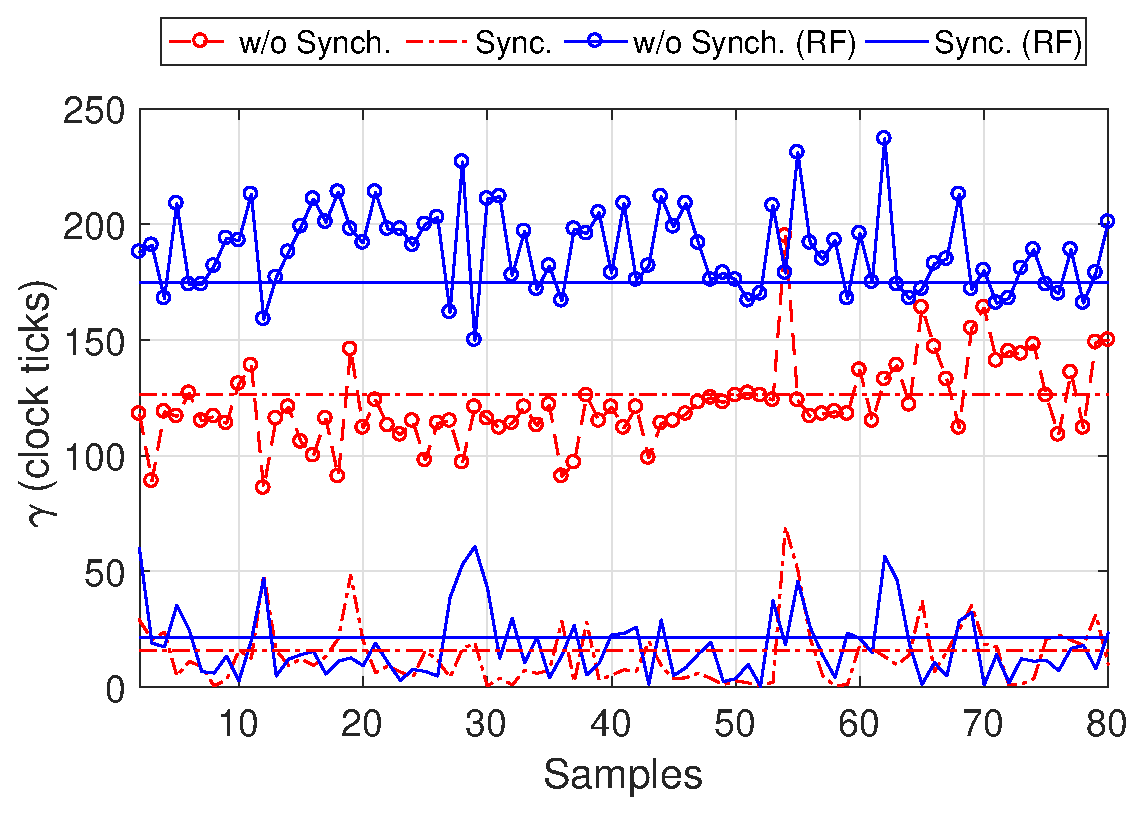
\includegraphics[width=0.9\columnwidth]{figures/synchronization_accuracy.eps}
	\caption{\label{fig:sync_error}Event-based synchronization performance when the tag is powered through a constant voltage source and through RF power. Mean synchronization errors without and with WISP-Sync were almost 127 and 16 clock ticks under stable voltage, and 175 and 22 clock ticks with RF power harvesting (represented by the straight lines in this figure), respectively.}
\end{figure}

Fig.~\ref{fig:sync_error} presents the synchronization error measurements when the tag is powered by using a constant voltage source, and powered only by an RFID reader. Measurements under constant and stable voltage allowed us to observe synchronization under stable clock frequency. We obtained a significant synchronization performance with WISP-Sync---almost a factor of eight less synchronization error as compared to the case where we did not perform any synchronization. It should be noted that even in this case, we observed quite fluctuating synchronization errors due to the varying transmission delays, that led a peak error to appear between samples 50 and 60. Apart from experiments with constant voltage input, measurements under highly varying RF power led us to observe the behavior of synchronization under highly varying clock frequencies. In this case, there is a considerable amount of increase on the error, i.e. approximately twice as much, as compared to the stable voltage case. However, we also obtained considerable improvements with our approach with unstable clock frequencies. WISP-Sync was quite reactive to the frequently varying clock frequencies and provided almost a factor of eight better accuracy.

\subsection{Power Loss and Recovery}

\begin{figure}
	\centering
	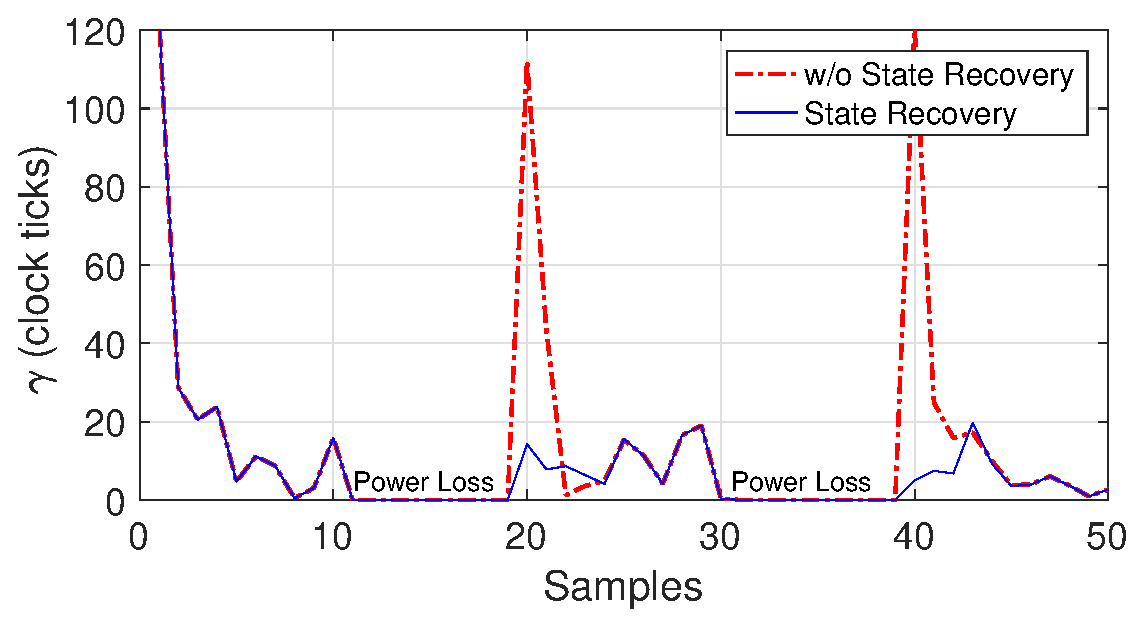
\includegraphics[width=0.85\columnwidth]{figures/power_loss.eps}
	\caption{\label{fig:power_loss}Impact of the state recovery on the synchronization performance. During the power loss periods, the tag is assumed to be turned off. With state recovery, presented by the solid line, the relative clock frequency is assumed to be saved in the FRAM and recovered back when sufficient power is supplied. On the other hand, the dashed line represents the case of starting synchronization from scratch. It can be observed that with state recovery, the tag adapts itself quickly and synchronization performance is considerably better, i.e. more than 100 clock ticks less synchronization error on power loss.} 
\end{figure}

In order to evaluate the performance of WISP-Sync under power losses, we simulated power loss in MATLAB by omitting the collected clock readings during predefined time intervals. As presented in Fig.~\ref{fig:power_loss}, after samples 10 and 30 WISP-Sync is disabled and before the beginning of the sample times 20 and 40 the algorithm is enabled. The solid line in this figure indicates enabling algorithm with state recovery, where the algorithm starts to execute using the value of $\hat{f}_w^r$  previously saved in the FRAM before power loss. It is apparent that with state recovery, the tag quickly adapts itself and re-synchronization is quickly established. On the other hand, starting the algorithm from scratch, as presented by the dashed lines, is problematic since it takes several steps to re-synchronize the tag.
%
%\begin{figure}
%		\begin{lstlisting}[style = mystyle,escapechar=|] 
%		_attribute_((section(".infoA"))) float f_w = 0.0f;
%		uint16_t t_f = 0;
%		
%		void wisp_sync(uint16_t c_w) {
%			float error = (float)c_w - ((float)t_f + TAU * (1.0f + f_w));
%			f_w += BETA * error;
%		}
%		\end{lstlisting}
%\caption{The actual implementation of  lines 3--5 of Algorithm~\ref{alg:sync} in C language for TI MSP430FR5969 platform. Constants \texttt{BETA} and \texttt{TAU} are defined outside of this function in the remaining part of the C program implementing Algorithm~\ref{alg:sync}.}
%		\label{fig:wisp_implementation}
%\end{figure}
%
\subsection{Energy Overhead}
%
We now present the real energy measurements of the actual WISP tag-side C language implementation of lines 3--5 of Algorithm~\ref{alg:sync} which are the main computation steps to calculate the new values of the variables pertaining to the synchronization. We performed our measurements using the Energy-interference-free Debugger (EDB)~\cite{colin2016energy} to measure the output voltage without affecting the energy state of the tag. EDB charges the capacitor of a device to a certain level and then disconnects itself. Using this feature of EDB we charge the capacitor of WISP to 2.45\,V, i.e. just above the operational level of WISP. While the program is being executed, the value of the capacitor is measured at specific code locations---in this case before Line 3 and after Line 5 of Algorithm~\ref{alg:sync}. The difference between these two results represents the energy overhead of WISP-Sync. We repeated this experiment ten times to eliminate quantization effects during measurements. We observed an average energy of $\approx1.85 \mu$J with a standard deviation of 0.038\,$\mu$J is spent by the tag in order to perform the aforementioned computations.

The main source of energy consumption in our implementation is the \emph{floating point arithmetic}: WISP-Sync requires two multiplications, three additions and one subtraction on float variables. Since MSP430 microcontroller does not have any floating point coprocessor, the float operations are handled using a software library, that makes them relatively slow. We used the standard gcc compiler (specifically, msp430-gcc version 6.2.1.16) math library for the sake of the portability of float operations. However, we expect that a more efficient architecture-specific implementation of the math library in software or an architecture with a math coprocessor will lead to less computation time and in turn relatively less energy overhead for WISP-Sync~\cite{mathlib_website}. Another point we would like to mention is that non-volatile memory access consumes more power as compared to SRAM access~\cite[Section 3.3]{ti_fram}. The only non-volatile variable in WISP-Sync is $\hat{f}_w^r$ in Algorithm~\ref{alg:sync}. This variable is read twice but modified once in our implementation. On the other hand, WISP-Sync maintains only one variable in SRAM, i.e. $t_f$, which is read only once. We conclude that WISP-Sync performs three FRAM and one SRAM access operations---low energy overhead in terms of memory access.

\subsection{Limitations of WISP-Sync}

In conclusion, the experimental results so far indicated that a maximum synchronization error of approximately 1.5 ms can be ensured between an RFID reader and a single WISP tag when employing event-based synchronization. The main factors that limited the WISP-Sync synchronization accuracy were the clock precision of the WISP platform and the non-deterministic transmission delays during reader-tag communication. As we indicated, we used the external 32\,kHz clock of the platform since it is also running when the tag is in very low-power operation mode. Therefore, in the best case when there are no transmission delays, the quantization effect due to the timing measurements using the low precision clock will not allow a better synchronization accuracy than 32\,$\mu$s. On the other hand, to obtain this synchronization accuracy with WISP-Sync, the reader and the tags shoud support a high-precision and accurate packet timestamping as in sensor networks~\cite{Maroti2004}. As indicated in Section \ref{sec:CRFIDs}, the effect of the non-deterministic delays should be reduced for a better synchronization accuracy.

Even though the event-based approach is relatively lightweight and adaptive as compared to the sender-receiver synchronization, it has some limitations. First, the tag is unable to obtain an \emph{explicit reference clock value}. The only variable it tunes is the $\hat{f}_w^r$ that represents the relative frequency of the software clock with respect to the clock of the reader. Therefore, we require additional steps that will allow tags to obtain the actual reference clock value. \add{Moreover, if the tags are covered by different readers, the first step should be to first synchronize the readers to the real-time. e.g. by allowing them to access time servers using internet.}
%However, to the best of our knowledge, there is no such command in the EPC Gen 2 standard that allows to send the explicit RFID reader time to the tag.
Second, WISP-Sync requires knowledge about $\tau$, which can be RFID reader dependent and requires a sniffer setup described in Section~\ref{sec:sniffer} to measure. This limitation can be addressed by employing an iterative estimation as an initial step to the WISP-Sync: the tag can start with an initial estimated $\tau$ value, and improve its estimation as it receives successive packets from the reader. After some iterations, the tag can have a rough estimate $\hat{\tau}$ that can be used on behalf of $\tau$. However, estimation errors might also perturb the synchronization accuracy. Last, the steps in Fig.~\ref{fig:event_based} present the communication scenario between one WISP and the reader. To allow other tags sniff this communication and synchronize, a broadcast primitive is crucial---in the next section we show how to overcome this limitation.

\section{The Synchronization of Multiple WISP Tags Using the WISP-Sync}
\label{sec:multi-wisp}

In this section, we turn our attention to the synchronization of  multiple WISP tags using the WISP-Sync. To this end, we have done the \emph{real implementation} of the WISP-Sync using the C programming language and TI's CCS~\cite{ti_css}, instead of using MATLAB to simulate our protocol using the collected the clock values from our testbed. Moreover, we extended our experimental testbed in Section~\ref{sec:testbed} by introducing two additional tags, as presented in Fig.~\ref{fig:testbed-new}. 


\begin{figure}
	\centering
	\begin{tikzpicture}
	\node[anchor=south west, inner sep=0] at 
	(0,0){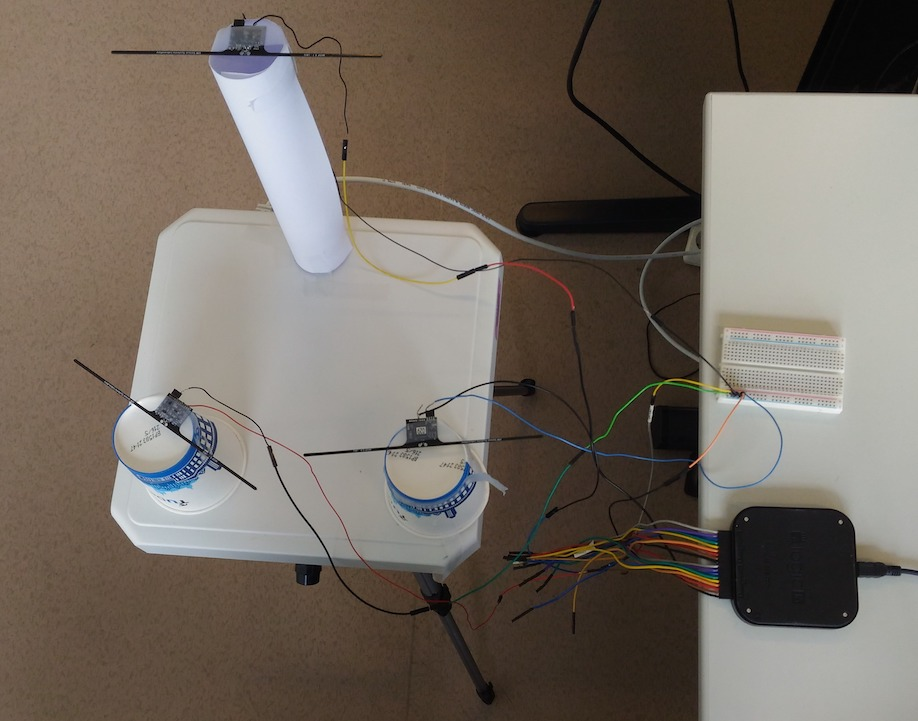
\includegraphics[width=0.8\columnwidth]{figures/3-wisps_resized.jpg}};
	
	\node [fill= white,circle] at (0.8,2.5) { };
	\node [color=black ] at (0.8,2.5) { 1 };
	
	\node [fill= white,circle] at (1,5.1) {  };
	\node [color=black ] at (1,5.1) { 2 };
	
	\node [fill= white,circle] at (2.3,2.1) {  };
	\node [color=black ] at (2.3,2.1) { 3 };
	
	\node [fill= white,circle] at (5.5,1) {  };
	\node [color=black ] at (5.5,1) { 4 };
	
	\node [fill= white,circle] at (5.5,2.8) {  };
	\node [color=black ] at (5.5,2.8) { 5 };
	
	\end{tikzpicture}
	\caption{\label{fig:testbed-new} A testbed of multiple tags: (1,2,3) tags, (4) logic analyzer, (5) breadboard. Tags 1 and 3 were at 8\,cm while tag 2 was at 20\,cm distance to the reader. The breadboard was used to make connections between the logic analyzer and the tags.} 
\end{figure}

We programmed the RFID Reader to send synchronization points via \emph{BlockWrite} command with a period of one second and we programmed two tags using our WISP-Sync implementation. On the other hand, we disabled clock synchronization for the last tag---which was a baseline for our evaluation.  In order to allow tags to simultaneously receive the information sent by the RFID Reader, we exploited an overhearing mechanism presented first in ~\cite[Section III-B]{stork:2017}. Therefore, during the experiments in our testbed (i) all of the tags received the periodic synchronization points sent by the RFID Reader; (ii) only two tags process this information and run Algorithm~\ref{alg:sync} to update their software clocks; (iii) the last tag did not participate in synchronization.

In order to measure the synchronization accuracies of the tags, we configured one of the ports of the MSP430 microcontroller as an output port and let tags (i) to set this port when they receive the first \emph{BlockWrite} command in Algorithm~\ref{alg:sync} (Line 1); (ii) to set a timer that will fire at their predicted time of the reception of the last \emph{BlockWrite} command from the RFID Reader; (iii) to clear this port when their timer fires. We connected the output ports to logic analyzer~\cite{saleae} and measured the time difference between the times at which the output ports are cleared. This allowed us to measure the prediction errors among the tags. We observed that all the tags set their output ports when they overhear the first \emph{BlockWrite} command, however their clear times are quite different and depend on their prediction error---the port clear times of the synchronizing two tags were closer to each other while they were quite different than the unsynchronized tag.

\begin{figure}
	\centering
	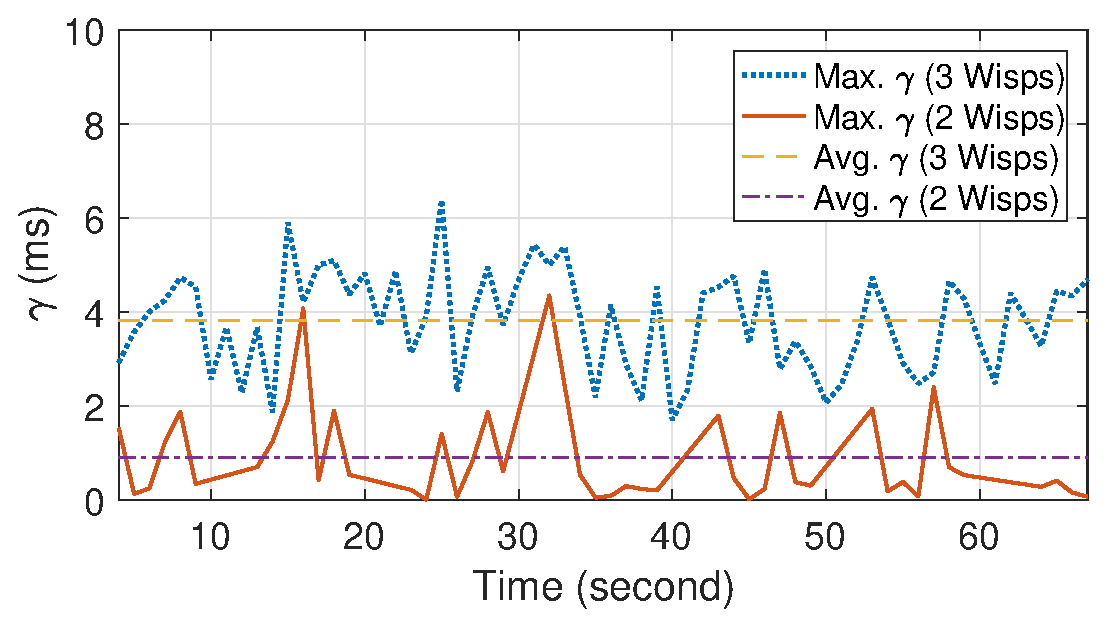
\includegraphics[width=0.9\columnwidth]{figures/multiwisp-experiments.eps}
	\caption{\label{fig:multi-sync-results}The synchronization error calculated during the experiments in our testbed. The blue dotted line denotes the maximum synchronization error among all of the tags (including the one which did not participate in synchronization) whereas the red line denotes the maximum error just between the synchronized tags.} 
\end{figure}

In Fig.~\ref{fig:multi-sync-results}, we plotted two different results: (i) the blue line depicts the maximum synchronization error (i.e. the maximum pairwise difference between the port clear times) when we considered all of the tags; (ii) the red line depicts when only synchronized tags are considered. From this figure it can be concluded that synchronization led to a factor of approximately four times better prediction on average among the tags: we observed an average synchronization error of 1\,ms while it was 4\,ms when one of the tags was unsynchronized.  

\section{Conclusions and Future Research Directions}
\label{sec:Conclusion}

In this article we explored synchronization scenarios between an RFID reader and WISP tags. We studied sender-receiver and event-based synchronization mechanisms in this setting and provided initial designs that will guide future explicit synchronization mechanisms among individual WISPs that reside inside the communication range of a common RFID reader. We provided implementation and evaluation of these designs in our testbed and identified their limitations and drawbacks. Our main finding is that with lightweight mechanisms, as of now, an average synchronization error of approximately 1\,ms can be ensured among tags. We provide the following issues for future studies in this domain:

\begin{itemize}
	\item \textbf{Network-wide synchronization:} We studied event-based synchronization among many tags. However, synchronization of these tags where they can access the explicit clock of the RFID reader and also synchronization of the whole CRFID network composed of several RFID readers and tags is still an issue, due to the single-hop nature of backscatter communication. Since tags can only communicate with the reader, not with their neighboring tags, it is interesting to explore \emph{WISP to WISP} synchronization. 
	
	\item \textbf{Power loss and recovery:} It is crucial to save the synchronization status to non-volatile memory just before the power loss, but writing to non-volatile memory also consumes energy. Hence, when to save the synchronization status without extra hardware support is worth exploring~\cite{Buettner:2011:Dewdrop,Ransford:2011:Mementos,Lucia:2015:Execution,Colin:2016:Debugger}.
	
	\item \textbf{Voltage-frequency relations:} It might be interesting to explore the voltage-clock frequency relationship since1 tags are subject to varying voltage source when they are powered with only RF energy harvesting from the RFID reader. We anticipate that voltage level should be incorporated to the establishment of the software clock so that voltage dependent instability of clock frequency can be compensated. However, this is a ``chicken or egg'' problem since reading the voltage level also consumes energy. 
	
	\item \textbf{Synchronization in other IPD platforms:} Synchronization in other IPD platforms, e.g. that use ambient backscatter communication \cite{ambient_backscatter}, is worth exploring as well. 
\end{itemize}

\ifCLASSOPTIONcaptionsoff
  \newpage
\fi

\bibliographystyle{IEEEtran}
\bibliography{IEEEabrv,references}

\newpage\null\thispagestyle{empty}\newpage
\appendices
\section{Analysis of Algorithm~\ref{alg:sync}}

We provide the synchronization conditions of Algorithm~\ref{alg:sync} and show that the synchronization will be established eventually. We need to mention that we follow similar calculation steps to the ones presented in the studies~\cite{pi2015,Yildirim:Gradient:2016}. However, since we use a different clock drift model in this article, i.e. Brownian motion rather than uniform distribution, the following  mathematical analysis is moderately different and more realistic as compared to those in the previous studies. 

Since $f_w$ and $f_r$ are time varying, by following 
\cite{Zhong:2011:On-demand,Huang:2013:PSR}, we model the 
\emph{evolution} 
of $f_w^r$ as 
integrated white noise, i.e. \emph{Brownian motion}, given as
\begin{eqnarray}
f_{w}^{r}(t_{0}+\delta) & \triangleq & 
f_{w}^{r}(t_{0})+\int_{t_{0}}^{t_{0}+\delta}\eta(t)dt.\label{eq:drift}
\end{eqnarray}
Here, $\delta$ denotes the amount of time after $t_0$ and $\eta(t)$ denotes 
the instantaneous change on the relative clock frequency, namely 
\emph{relative drift rate} at time $t$. We assume that 
$\eta(t)\sim\mathcal{N}(0,\sigma_{\eta}^{2})$ and for all 
time instants $t'$ and $t''$, $\eta(t')$ and $\eta(t'')$ are uncorrelated 
random variables. In order to ease the calculations in the following sections, 
we will consider the \emph{average relative clock frequency} in an interval of 
interest $[t_0,t_0+\delta]$ rather than instantaneous relative frequency 
in~\eqref{eq:drift}. We denote this value by $\bar{f}_{r}^{w}(t_0,t_0+\delta)$ 
and define it as 
\begin{eqnarray}
\bar{f}_{w}^{r}(t_0,t_0\!+\!\delta) &\!\!\!\!\! \triangleq\!\!\!\!\! & 
\frac{1}{\delta}\!\!\int_{t_0}^{t_0+\delta}\!\!\!\!\!\!\!\!\!\!\!\! 
f_w^r(t)dt \triangleq
f_{w}^{r}(t_{0})\!+\!\frac{1}{\delta}\!\!\int_{0}^{\delta}\!\!\int_{t_{0}}^{t_{0}+t}\!\!\!\!\!\!\!\!\!\!\!\eta(u)dudt.
\label{eq:drift_relation}
\end{eqnarray}


\subsection{Proof of Convergence}
Consider \eqref{eq:gamma_t_1} and without loss of 
generality we assume that 
$C_{w}(t_{1})-C_{w}(t_{0})=\tau(1+\bar{f}_{w}^{r}(t_0,t_1))+\varepsilon$
where $\tau$ denotes the event period and $\varepsilon$ accounts for the 
uncertainty of the event period (as 
indicated in Section \ref{subsec:event_period_uncertainty}). For ease of 
calculations we assume that $\varepsilon\sim\mathcal{N}(0,\sigma^2_{\tau})$. 
Define \emph{relative frequency estimation error} as
\begin{eqnarray}
\tilde{f}_{w}^{r}(t_0) & \triangleq & 
f_{w}^{r}(t_0)-\hat{f}_{w}^{r}(t_0).\label{eq:relative_drift_estimation_error}
\end{eqnarray}
Using \eqref{eq:gamma_t_1}, \eqref{eq:drift_relation} and 
\eqref{eq:relative_drift_estimation_error} we get:
\begin{eqnarray}
\gamma(t_1) & = & 
\tau(\bar{f}_{w}^{r}(t_0,t_1)-\hat{f}_{w}^{r}(t_0))+ \varepsilon \nonumber \\
&=&  
\tau\tilde{f}_{w}^{r}(t_0)+\frac{\tau}{t_1-t_0}\int_{0}^{t_1-t_0}\!\!\!\int_{t_{0}}^{t_0+t}\!\!\!\!\!\!\!\!\!\!\!\eta(u)dudt
+ \varepsilon.
\end{eqnarray}
For ease of representation, let us introduce the following 
notation:
\begin{eqnarray}
\Phi(h) &\triangleq& \int_{t_h}^{t_{h+1}}\eta(t)dt, \\
\Omega(h) &\triangleq& 
\frac{\tau}{t_{h+1}-t_h}\int_{0}^{t_{h+1}-t_h}\int_{t_{h}}^{t_h+t}\eta(u)dudt,
\\
\Delta(h) &\triangleq& \tilde{f}_{w}^{r}(t_{h}). \label{eq:delta}
\end{eqnarray}
Using this notation, we denote $\gamma(t_{h+1})$ by $\Theta(h+1)$ as
\begin{eqnarray}
\Theta(h+1) &\triangleq& \gamma(t_{h+1})=\tau\Delta(h) + \Omega(h)+\varepsilon. 
\label{eq:theta}
\end{eqnarray}
Moreover, since $\Delta(h)$, $\Omega(h)$ and $\varepsilon$ are 
independent random variables, we can write $\Delta(h+1)$ as
\begin{eqnarray}
\Delta(h+1) &\overset{\eqref{eq:delta}}{=}& 
\Delta(h)+\tilde{f}_{w}^{r}(t_{h+1})-\tilde{f}_{w}^{r}(t_{h}) \nonumber \\
&\overset{\eqref{eq:relative_drift_estimation_error}}{=}& \Delta(h)
\!+\!f_w^r(\!t_{h+1}\!)\!-\!\!f_w^r(\!t_{h}\!) \!-\!\!\hat{f}_w^r(\!t_{h+1}\!)\!+\!\!\hat{f}_w^r(\!t_{h}\!)
\nonumber\\
&\overset{\eqref{eq:update_rule},\eqref{eq:drift}}{=}& 
\Delta(h)+\int_{t_h}^{t_{h+1}}\eta(t)dt-\beta\Theta(h+1) \nonumber \\
&\overset{\eqref{eq:theta}}{=}& 
(1-\beta\tau)\Delta(h)-\beta(\Omega(h)+\varepsilon) +\Phi(h). 
\label{eq:delta_recursive}
\end{eqnarray} 
Considering \eqref{eq:theta} and \eqref{eq:delta_recursive}, we can write the 
system evolution as
\begin{eqnarray}
\underset{X(h+1)}{
	\underbrace{
		\left[\!\!\!\begin{array}{c}
		\Theta(h\!+\!1)\\
		\Delta(h\!+\!1)
		\end{array}\!\!\!\right]
	}
} &\!\!\!\!\!\!\! =\!\!\!\!\!\!\! & 
\underset{A}{
	\underbrace{
		\left[\!\!\!\begin{array}{cc}
		0 & \tau\\
		0 & 1\!-\!\beta\tau
		\end{array}\!\!\!\right]
	}
}
\underset{X(h)}{
	\underbrace{
		\left[\!\!\!\begin{array}{c}
		\Theta(\!h\!)\\
		\Delta(\!h\!)
		\end{array}\!\!\!\right]}
}
\!\!+\!\!
\underset{Y(h)}{
	\underbrace{
		\left[\!\!\!\begin{array}{c}
		\Omega(h)+\varepsilon\\
		\Phi(\!h\!)\!-\!\beta(\Omega(\!h\!)\!+\!\varepsilon)
		\end{array}\!\!\!\right]}
}.\label{eq:state_space-pi}
\end{eqnarray}
Taking the expectation of both sides of \eqref{eq:state_space-pi} yields 
$\expected{X(h+1)} = A\expected{X(h)}$ since 
the means of the random variables in the matrix $Y(h)$ are all zero. According 
to stability of linear systems \cite{book-luenberger}, \emph{asymptotic 
	convergence} will be reached if and only if the magnitudes of the 
eigenvalues of the matrix $A$ are strictly smaller than one. The eigenvalues 
$\lambda_1$ and $\lambda_2$ of the matrix $A$ can be obtained 
by solving
\begin{eqnarray}
\left|\begin{array}{cc}
-\lambda & \tau\\
0 & 1-\beta\tau-\lambda
\end{array}\right|=0 &\implies& 
\begin{array}{c}
\lambda_1 = 0,\\
\lambda_2 = 1-\beta\tau.  
\end{array}\label{eq:eigens}
\end{eqnarray}
Therefore, the synchronization will be  established if 
and only if $|\lambda_1,\lambda_2|<1$, and in turn
\begin{align}
0 & <\beta<\frac{2}{\tau}\label{eq:step_size_bounds-pi}
\end{align}
should hold. The 
rate of convergence is governed by 
the largest eigenvalue $\lambda_2$, which means that bigger values of $\beta$ 
will lead to faster convergence. 
Consequently, selecting $\beta$ within the bound above will lead the system  
converge to the state  
\begin{eqnarray}
\underset{h\rightarrow\infty}{\lim}\expected{\Theta(h+1)} &=&
\expected{\Theta(h)}, \label{eq:asymp_theta} \\
\underset{h\rightarrow\infty}{\lim}\expected{\Delta(h+1)}&=&
\expected{\Delta(h)} \label{eq:asymp_delta}.
\end{eqnarray}
Hence, due to asymptotic convergence
\begin{eqnarray}
\expected{\Delta(\infty)} \overset{\eqref{eq:delta_recursive}}{=} 
\left(1-\beta 
\tau\right)\expected{\Delta(\infty)} &\!\!\!\!\!\!\!\implies\!\!\!\!\!\!\!& \expected{\Delta(\infty)}\!=\!0, 
\label{eq:delta_convergence}\\
\expected{\Theta(\infty)}  \overset{\eqref{eq:theta}}{=} 
\tau\expected{\Delta(\infty)}&\!\!\!\!\!\!\!\implies\!\!\!\!\!\!\!&\expected{\Theta(\infty)}\!=\!0. 
\label{eq:expected_error}
\end{eqnarray}
Consequently, the prediction error $\Theta(h)=\gamma(t_h)$ 
eventually converges to zero as $h$ goes to infinity. This means the WISP tag 
will estimate the occurrence times of the successive
events with zero error in expectation. 


\subsection{Steady-State (Asymptotic) Synchronization Error}
\label{sec:app_b}
An analytical expression for the \emph{asyptotic 
	synchronization error} can be obtained by calculating 
$\underset{h\rightarrow \infty}{\lim}\mathrm{Var}(\Theta(h))$. This 
calculation reduces to find 
$\mathrm{Var}(\Theta(\infty))=\expected{\Theta(\infty)^2}$, since it holds 
from 
\eqref{eq:expected_error} that $\expected{\Theta(\infty)}=0$. Using 
\eqref{eq:theta}, we 
get
\begin{eqnarray}
\expected{\Theta(\infty)^2} &\!\!\!\!\overset{\eqref{eq:theta}}{=}\!\!\!\!& 
\tau^2\expected{\Delta(\infty)^2}  
+\expected{(\Omega(h)+\varepsilon)^2},\label{eq:expected_theta_infinity}
\end{eqnarray}
since $\expected{\Delta(\infty)}=0$ from \eqref{eq:delta_convergence} and 
$\Delta(h)$, $\Omega(h)$ and $\varepsilon$ are independent. 
In order to calculate \eqref{eq:expected_theta_infinity}, let us derive first 
$\expected{\Delta(\infty)^2}$ as
\begin{eqnarray}
\!\!\!\!\!\expected{\!\Delta(\!\infty\!)^2\!} 
&\!\!\!\!\!\!\!\overset{\eqref{eq:delta_recursive},\eqref{eq:asymp_delta}}{=}\!\!\!\!\!\!& 
(\!1\!\!-\!\!\beta\tau\!)^2\!	
\expected{\!\Delta(\!\infty\!)^2}  
\!\!+\!\!\expected{\!(\!\Phi(\!h\!)\!\!-\!\!\beta\!(\!\Omega(\!h\!)\!+\!\varepsilon\!)^2}\!. 
\label{eq:expected_delta_infinity}
\end{eqnarray}
In order to calculate \eqref{eq:expected_delta_infinity}, the first step is to 
obtain the following expectation:
\begin{eqnarray}
\expected{(\Phi(h)\!-\!\beta(\Omega(h)\!+\!\varepsilon)^2} 
&\!\!\!\!=\!\!\!\!&
\expected{(\Phi(h)^2}
\!-\!2\beta\expected{\Phi(h)\Omega(h)} 
\! \nonumber \\ 
& & +\!\beta^2\expected{\Omega(h)^2}\!+\!\beta^2\expected{\varepsilon^2}. 
\label{eq:stochastic_expectation}
\end{eqnarray}
The equality \eqref{eq:stochastic_expectation} holds due to the fact that 
$\expected{\Phi(h)\varepsilon}=\expected{\Phi(h)}\expected{\varepsilon}=0$ and 
$\expected{\varepsilon\Omega(h)}=\expected{\varepsilon}\expected{\Omega(h)}=0$ 
(since 
$\expected{\varepsilon}=\expected{\Phi(h)}=\expected{\Omega(h)}=0$ and 
$\varepsilon$ is independent from $\Phi(h)$ and $\Omega(h)$). The
following \emph{stochastic integrals} are required for 
\eqref{eq:stochastic_expectation}:
\begin{eqnarray}
\expected{\Phi(h)^2}\!\!\!\!\!\!\! 
& = & \!\!\!\!\!\!
\int_{0}^{t_{h+1}-t_h}\!\!\!\!\!\!\!\!\!\!\!\!\!\!\!\!\!\!\sigma_{\eta}^{2}dt =  \sigma_{\eta}^{2}(t_{h+1}-t_h),\\
\expected{\Omega(h)^2}\!\!\!\!\!\!\! 
& = & \!\!\!\!\!\!
\frac{\tau^2}{(t_{h+1}\!\!-\!\!t_h)^2}
\sigma_{\eta}^{2}\!\!\!\int_{0}^{t_{h+1}-t_h}\!\!\!\!\!\!\!\!\!\!\!\!\!\!\!\!\!\!\!t^2dt\! = \!
\sigma_{\eta}^{2}\!\frac{\tau^2(\!t_{h+1}\!\!-\!\!t_h\!)}{3},\label{eq:stochastic_integral}\\
\expected{\Phi(h)\Omega(h)}\!\!\!\!\!\!\! 
& = & \!\!\!\!\!\!
\frac{\tau}{t_{h+1}-t_h}\sigma_{\eta}^{2}\int_{0}^{t_{h+1}-t_h}\!\!\!\!\!\!\!\!\!\!\!\!\!\!\!\!\!\!tdt = 
\sigma_{\eta}^{2}\frac{\tau(\!t_{h+1}\!\!-\!\!t_h\!)}{2}, \\
\expected{\varepsilon^2}\!\!\!\!\!\!\! 
& = & \!\!\!\!\!\! 
\sigma_{\tau}^{2}.
\end{eqnarray}	
The derivation of the expectations and stochastic integrals above relies on the 
assumptions we mentioned 
at the beginning of this Appendix: (i) $\eta(t')$ and $\eta(t'')$ are 
uncorrelated for all $t'\neq t''$, therefore $\expected{\eta(t')\eta(t'')}=0$; 
(ii) since $\expected{\eta(t')}=0$, therefore 
$\expected{(\eta(t'))^2}=\mathrm{Var}(\eta(t'))=\sigma_{\eta}^2$. Putting these 
expected 
values into \eqref{eq:stochastic_expectation}, then in 
turn into \eqref{eq:expected_delta_infinity} lead:
\begin{eqnarray}
\expected{\Delta(\infty)^2}\!\!\!\!\!\!
& = &\!\!\!\!\!\!
\frac{\sigma^2_{\eta}(t_{h+1}-t_h)\left(1-\beta\tau+\frac{\beta^2\tau^2}{3}\right)\!\!+\!\!\beta^2\sigma^2_{\tau}}{(2\beta\tau-\beta^2\tau^2)}.
\label{eq:delta_infinity}
\end{eqnarray}
Finally, putting \eqref{eq:delta_infinity} into 
\eqref{eq:expected_theta_infinity} 
leads to
\begin{eqnarray}
\expected{\Theta(\infty)^2}\!\!\!\!\!\!\! & = & \!\!\!\!\!\!\!
\frac{\sigma^2_{\eta}(t_{h+1}-t_h)\left(\tau^2
	-\beta\tau^3-\frac{\beta^2\tau^4}{3}\right)
	+\beta^2\sigma^2_{\tau}\tau^2}{(2\beta\tau-\beta^2\tau^2)} \nonumber \\ 
\!\!\!\!\!\!\! &  & \!\!\!\!\!\!\!+ 
\sigma^2_{\eta}\frac{\tau^2(t_{h+1}-t_h)}{3}+\sigma^2_{\tau}.
\end{eqnarray}
Without loss of generality, assume that $t_{h+1}-t_h\approxeq\tau$. Therefore, 
the asymptotic estimation error of Algorithm \ref{alg:sync} is given by
\begin{eqnarray}
Var\left(\underset{h\rightarrow\infty}{\gamma(t_h)}\right)\!\!\!\!\!\!\!& = &\!\!\!\!\!\! 
\expected{\Theta(\infty)^2}\!\! = \!\!
\frac{\sigma^2_{\eta}\left(\tau^2-\beta\tau^3
	+\frac{\beta^2\tau^4}{3}\right)
	+\beta^2\sigma^2_{\tau}\tau}{(2\beta-\beta^2\tau)} \nonumber \\
\!\!\!\!\!\!\!& = &\!\!\!\!\!\!  +\frac{\sigma^2_{\eta}\tau^3}{3}
+  \sigma^2_{\tau}
\end{eqnarray}
which results in \eqref{eq:sync_performance}.


% biography section
% 
% If you have an EPS/PDF photo (graphicx package needed) extra braces are
% needed around the contents of the optional argument to biography to prevent
% the LaTeX parser from getting confused when it sees the complicated
% \includegraphics command within an optional argument. (You could create
% your own custom macro containing the \includegraphics command to make things
% simpler here.)
%\begin{IEEEbiography}[{\includegraphics[width=1in,height=1.25in,clip,keepaspectratio]{mshell}}]{Michael Shell}
% or if you just want to reserve a space for a photo:

%\begin{IEEEbiography}[{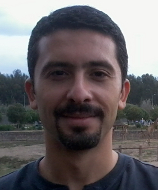
\includegraphics[width=1in,height=1.25in,clip,keepaspectratio]{author_photos/ksy.jpeg}}]{Kas{\i}m Sinan Y{\i}ld{\i}r{\i}m}
%received BSc(Eng), M.Sc. and Ph.D. degrees from Ege University, İzmir, 
%Turkey in 2003, 2006 and 2012 respectively. He is  currently with Embedded Software group of TU Delft. His research interests are embedded systems, distributed algorithms,  wireless sensor networks, energy harvesting systems and computational RFIDs.
%\end{IEEEbiography}
%
%% if you will not have a photo at all:
%\begin{IEEEbiographynophoto}{Henko Aantjes}
%Biography text here.
%\end{IEEEbiographynophoto}
%
%\begin{IEEEbiography}[{
\includegraphics[width=1in,height=1.25in,clip,keepaspectratio]{author_photos/przemek.jpg}}]{}
%Biography text here.	
%\end{IEEEbiography}
%
%\begin{IEEEbiography}[{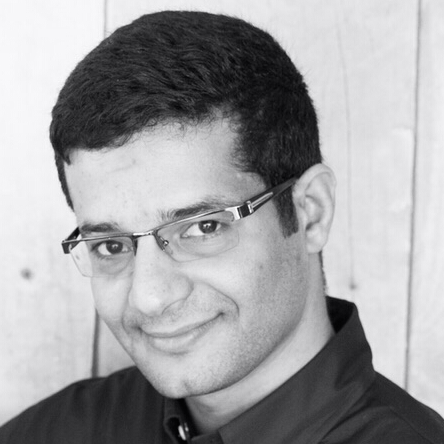
\includegraphics[width=1in,height=1.25in,clip,keepaspectratio]{author_photos/amjad.jpg}}]{Amjad Yousef Majid}
%Biography text here.
%\end{IEEEbiography}
%
% insert where needed to balance the two columns on the last page with
% biographies
%\newpage

% You can push biographies down or up by placing
% a \vfill before or after them. The appropriate
% use of \vfill depends on what kind of text is
% on the last page and whether or not the columns
% are being equalized.

%\vfill

% Can be used to pull up biographies so that the bottom of the last one
% is flush with the other column.
%\enlargethispage{-5in}



% that's all folks
\end{document}


